% Compile with XeLaTeX (Overleaf: Menu -> Compiler -> XeLaTeX); needed for the Vietnamese names on the cover.
% Figures are in figures/ (generated by make_figures.py and ../make_diagrams.py).
\documentclass[12pt,letterpaper]{article}

\usepackage[margin=1in]{geometry}
\usepackage{amsmath}
\usepackage{fontspec}
\usepackage{unicode-math}
\setmainfont{TeX Gyre Termes}
\setmathfont{TeX Gyre Termes Math}
\usepackage{graphicx}
\usepackage{booktabs}
\usepackage{array}
\usepackage{tabularx}
\usepackage{xcolor}
\usepackage{tikz}
\usepackage{caption}
\usepackage{enumitem}
\usepackage{titlesec}
\usepackage{placeins}
\usepackage[hidelinks]{hyperref}

\graphicspath{{figures/}}
\linespread{1.05}
\renewcommand{\contentsname}{TABLE OF CONTENTS}
\setlength{\parindent}{0pt}
\setlength{\parskip}{5pt}
\setlist{itemsep=2pt,topsep=3pt,parsep=0pt,leftmargin=1.4em}
\captionsetup{font=small,labelfont=bf,labelsep=period}
\setcounter{secnumdepth}{0}  % headings carry their own numbers, as in the template
\setcounter{tocdepth}{2}
\titleformat{\section}{\large\bfseries}{}{0pt}{}
\titleformat{\subsection}{\normalsize\bfseries}{}{0pt}{}
\titleformat{\subsubsection}{\normalsize\bfseries\itshape}{}{0pt}{}
\titlespacing*{\section}{0pt}{10pt}{4pt}
\titlespacing*{\subsection}{0pt}{8pt}{3pt}
\titlespacing*{\subsubsection}{0pt}{6pt}{2pt}
\renewcommand{\topfraction}{0.85}
\renewcommand{\bottomfraction}{0.7}
\renewcommand{\textfraction}{0.12}
\renewcommand{\floatpagefraction}{0.75}
\newcommand{\best}[1]{\textbf{#1}}

\begin{document}

% ------------------------------------------------------------------------------------------------ cover
\begin{titlepage}
\begin{tikzpicture}[remember picture,overlay]
  \draw[line width=3pt]
    ([xshift=0.75in,yshift=-0.75in]current page.north west) rectangle
    ([xshift=-0.75in,yshift=0.75in]current page.south east);
  \draw[line width=0.8pt]
    ([xshift=0.83in,yshift=-0.83in]current page.north west) rectangle
    ([xshift=-0.83in,yshift=0.83in]current page.south east);
\end{tikzpicture}
\centering
\vspace*{0.2in}
{\large\bfseries NATIONAL ECONOMICS UNIVERSITY\\[4pt] FACULTY OF MATHEMATICAL ECONOMICS\par}
\vspace{1.3in}
{\Large\bfseries MAJOR ASSIGNMENT\par}
\vspace{6pt}
{\large\bfseries Course: Deep Learning\par}
\vspace{0.6in}
{\LARGE\bfseries TOPIC:\par}
\vspace{14pt}
{\large\bfseries TIME-OF-DAY AND WEATHER CLASSIFICATION\\ OF DASHCAM IMAGES ON BDD100K\\
USING CONVOLUTIONAL NEURAL NETWORKS\par}
\vspace{0.7in}
\begin{flushleft}
\hspace*{0.9in}{\large\bfseries Instructor:} {\large\colorbox{yellow}{[Instructor name]}}\\[12pt]
\hspace*{0.9in}{\large\bfseries Students:}\\[4pt]
\large
\hspace*{0.9in}Nguyễn Trần Quốc Đạt -- \colorbox{yellow}{[Student ID]}\\
\hspace*{0.9in}Bùi Huỳnh Gia Huy -- \colorbox{yellow}{[Student ID]}\\
\hspace*{0.9in}Trương Đức Anh -- \colorbox{yellow}{[Student ID]}\\
\hspace*{0.9in}Ninh Duy Tuân -- \colorbox{yellow}{[Student ID]}
\end{flushleft}
\vfill
{\large\bfseries Hanoi, October 2026\par}
\vspace*{0.15in}
\end{titlepage}

\setcounter{page}{1}
{\small\tableofcontents}
\newpage

% ================================================================================================ PART 1
\section{PART 1: THEORY -- CONVOLUTIONAL NEURAL NETWORKS}

Convolutional neural networks (CNNs) are a family of deep neural networks designed for data with a grid-like
structure, such as images \cite{goodfellow2016}. Since LeNet-5 \cite{lecun1998}, and especially since AlexNet won
the ImageNet Large Scale Visual Recognition Challenge (ILSVRC) in 2012 \cite{krizhevsky2012}, CNNs have been the
standard tool for image classification, object detection and segmentation. This part reviews the theory behind the
models of Part~2: the convolution, activation, pooling and fully connected layers; how a CNN is trained and
regularized; the classic architectures from which the idea of a \emph{CNN block} comes; transfer learning; and the
evaluation metrics.

\subsection{1. From fully connected networks to CNNs}
A multilayer perceptron (MLP) treats an image as a flat vector. A $224\times224$ RGB image has 150{,}528 input values,
so a single fully connected layer with 1{,}000 hidden units already needs about 150 million weights. Such a layer
also ignores the two-dimensional structure of the image: neighbouring pixels are strongly correlated while distant
pixels are mostly independent, and the same pattern -- an edge, a headlight, a patch of sky -- can appear anywhere in
the frame. CNNs build these properties into the architecture through three ideas \cite{goodfellow2016,zhang2023}:
\begin{itemize}
  \item \textbf{Local connectivity.} Each output unit is connected only to a small neighbourhood of the input, its
        \emph{receptive field}, instead of to every pixel.
  \item \textbf{Weight sharing.} The same small set of weights (a \emph{kernel} or \emph{filter}) is applied at every
        spatial position, so the number of parameters does not depend on the image size.
  \item \textbf{Translation equivariance.} Because the kernel is shared, shifting the input shifts the output by the
        same amount; combined with pooling, the representation becomes approximately invariant to small shifts.
\end{itemize}
By stacking such layers, a CNN learns a hierarchy of features: the first layers respond to edges, colours and
textures, deeper layers combine them into parts and objects, and the receptive field grows with depth.
Figure~\ref{fig:overview} shows the typical structure: a \emph{feature extractor} made of convolution, activation
and pooling layers, followed by a \emph{classification head} of fully connected layers.

\begin{figure}[htbp]
\centering
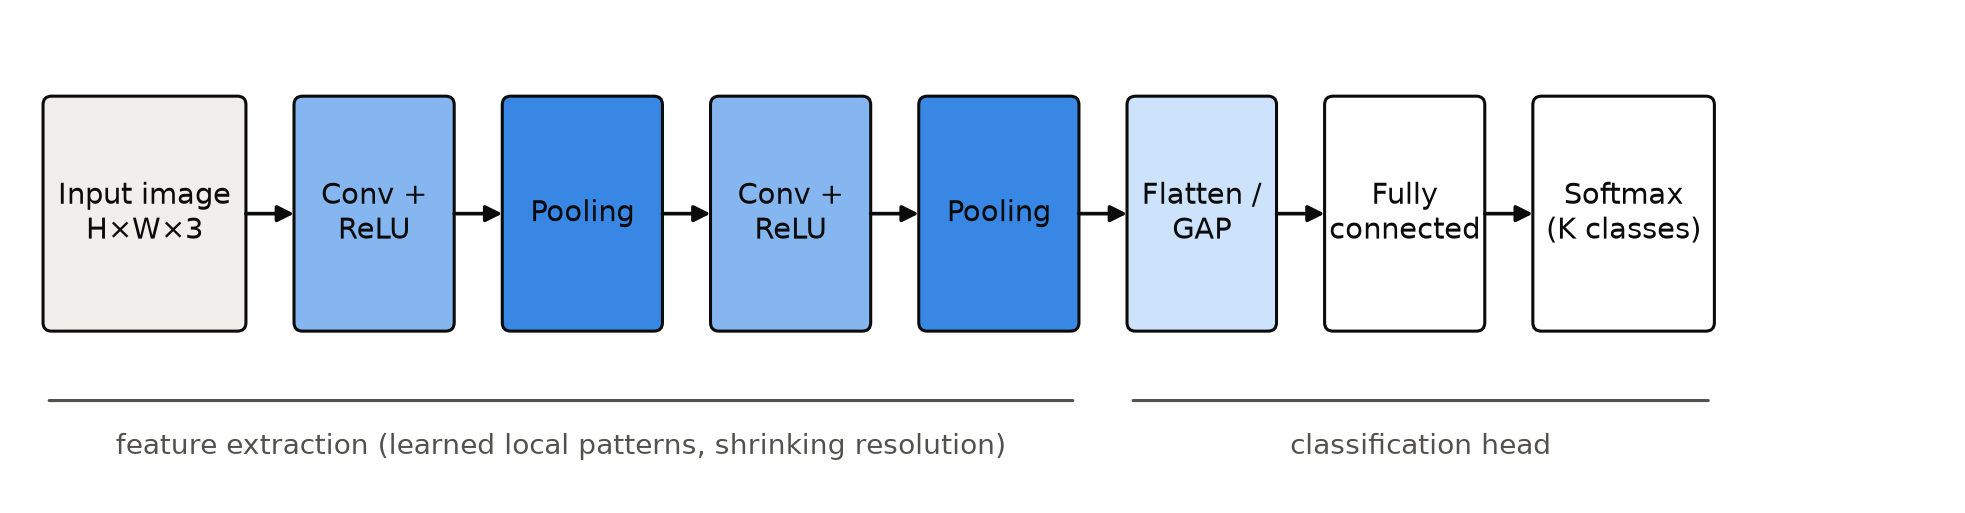
\includegraphics[width=0.92\textwidth]{cnn_overview.png}
\caption{General structure of a CNN for image classification.}
\label{fig:overview}
\end{figure}

\subsection{2. The convolutional layer}
\subsubsection{2.1. Convolution operation}
In deep learning libraries the ``convolution'' is in fact the cross-correlation between an input $X$ and a kernel
$W$ of size $k_h\times k_w$:
\begin{equation}
  Y[i,j] = \sum_{m=0}^{k_h-1}\sum_{n=0}^{k_w-1} X[i+m,\; j+n]\, W[m,n] + b .
  \label{eq:conv}
\end{equation}
The kernel slides over the input; at each position the element-wise products are summed and a bias $b$ is added,
giving one value of the output \emph{feature map} $Y$ (Figure~\ref{fig:conv}). The kernel weights are learned by
gradient descent, so the network itself decides which patterns to detect; whether the kernel is flipped (true
convolution) or not makes no difference, because the weights are learned anyway. Without padding and with stride
1, an $n_h\times n_w$ input gives an $(n_h-k_h+1)\times(n_w-k_w+1)$ output.

\begin{figure}[htbp]
\centering
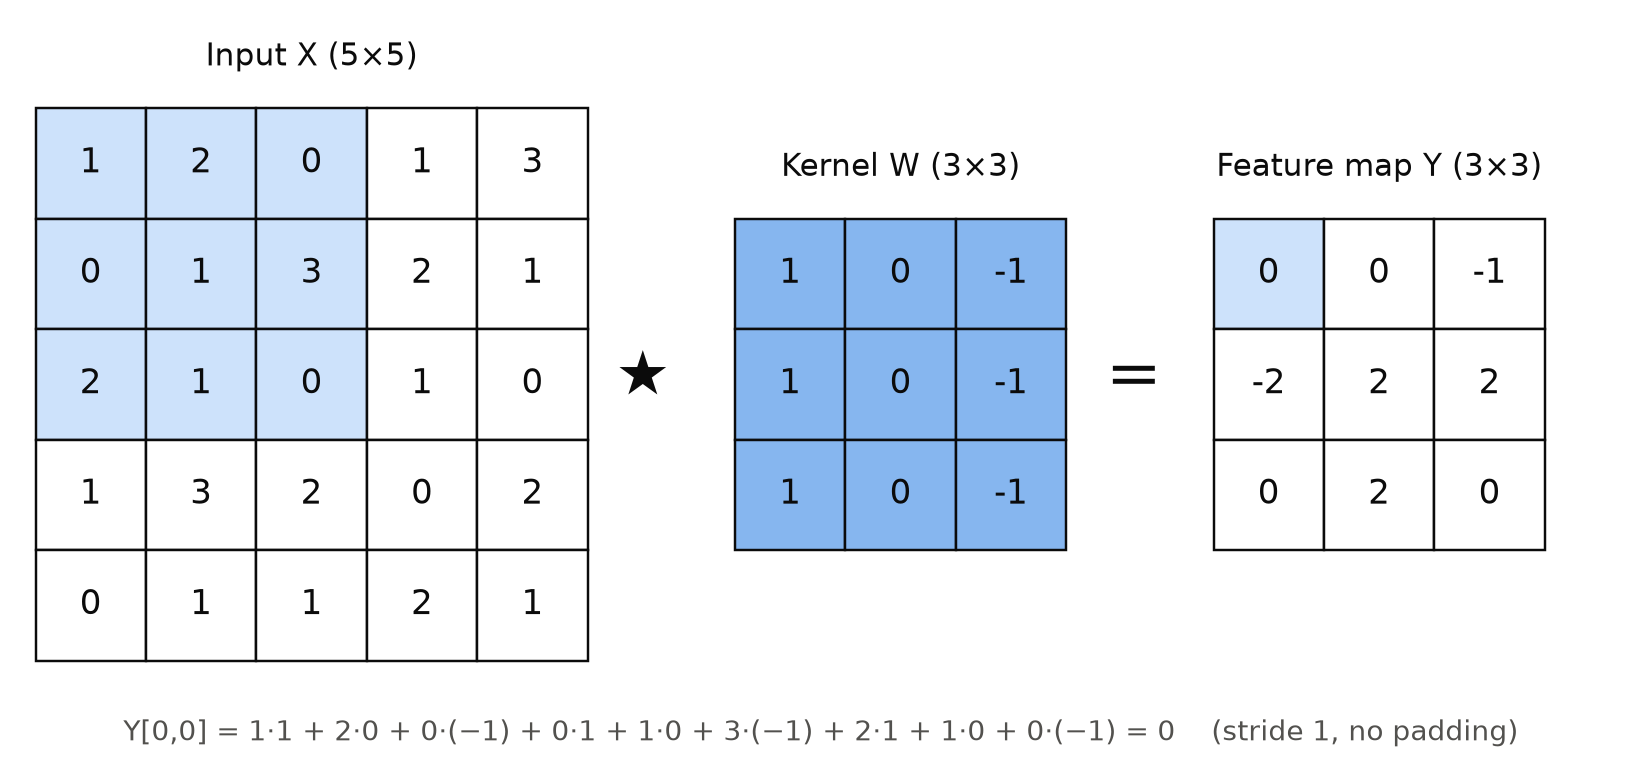
\includegraphics[width=0.66\textwidth]{convolution.png}
\caption{A 2-D convolution (cross-correlation) with a $3\times3$ kernel, stride 1 and no padding. The highlighted
window of the input produces the highlighted output value.}
\label{fig:conv}
\end{figure}

\subsubsection{2.2. Multiple channels and feature maps}
Real inputs have several channels (three for an RGB image) and a layer usually learns many kernels. A layer with
$C_{in}$ input and $C_{out}$ output channels has a weight tensor of shape $k_h\times k_w\times C_{in}\times C_{out}$:
the kernel of each output channel spans all input channels, the per-channel results are summed, and
\begin{equation}
  Y_o[i,j] = b_o + \sum_{c=1}^{C_{in}} \sum_{m,n} X_c[s\,i+m,\; s\,j+n]\, W_{o,c}[m,n],
  \label{eq:multi}
\end{equation}
where $s$ is the stride. Each output channel is a feature map that shows how strongly one learned pattern is present
at each location. The layer has $(k_hk_wC_{in}+1)\,C_{out}$ parameters, independent of the image size; for example,
the first layer of our simple CNN ($3\times3$ kernels, $3\rightarrow32$ channels) has $(3\cdot3\cdot3+1)\cdot32=896$
parameters, but it performs $9\cdot3\cdot32\cdot224\cdot224\approx43$ million multiply-adds, because the
computation, unlike the parameter count, grows with the resolution.

\subsubsection{2.3. Padding, stride and output size}
Without padding, every convolution shrinks the feature map by $k-1$ pixels and the border pixels are used less often
than the central ones. \textbf{Zero padding} adds $p$ rows and columns of zeros around the input; ``same'' padding
($p=\lfloor k/2\rfloor$ for an odd kernel and stride 1) keeps the spatial size unchanged, which is what all
$3\times3$ convolutions in our models use. The \textbf{stride} $s$ is the step of the sliding window: $s=2$ halves
the resolution and reduces the computation of the following layers about four times. For an input of height
$H_{in}$ the output height is
\begin{equation}
  H_{out} = \left\lfloor \frac{H_{in}+2p-k}{s} \right\rfloor + 1 ,
  \label{eq:size}
\end{equation}
and the width is computed in the same way. The complex CNN of Part~2 starts with a stride-2 convolution:
$\lfloor(224+2-3)/2\rfloor+1=112$.

\subsubsection{2.4. $1\times1$ convolutions}
A $1\times1$ convolution looks at a single pixel position but mixes all channels, i.e.\ it is a fully connected
layer applied independently at every location \cite{lin2014}. It is a cheap way to change the number of channels:
Inception and ResNet use it to reduce the channels before expensive $3\times3$ convolutions, and it matches the
channel count of a shortcut connection, as in the ConvBlock of our complex CNN.

\subsection{3. Activation functions}
Convolutions are linear; without a non-linearity, a stack of them would collapse into a single linear map. The
sigmoid $\sigma(z)=1/(1+e^{-z})$ used by LeNet saturates: its derivative is at most 0.25 and vanishes for large
$|z|$, so gradients shrink layer after layer in deep networks. The rectified linear unit
\cite{nair2010,krizhevsky2012}
\begin{equation}
  \mathrm{ReLU}(z)=\max(0,z)
  \label{eq:relu}
\end{equation}
is the default choice in CNNs: it is cheap to compute, its derivative is 1 for positive inputs, so gradients flow
well through deep networks, and it produces sparse activations. All hidden layers of our models use ReLU. For a
classification problem with $K$ classes, the last layer outputs $K$ scores (logits) $z_1,\dots,z_K$ that are turned
into a probability distribution by the softmax function
\begin{equation}
  \hat y_k = \frac{e^{z_k}}{\sum_{j=1}^{K} e^{z_j}}, \qquad k=1,\dots,K,
  \label{eq:softmax}
\end{equation}
and the predicted class is the one with the largest probability. In this project $K=6$.

\subsection{4. Pooling layers}
A pooling layer summarizes each small window of a feature map by a single number. It has no learnable parameters
and works on each channel separately, so the number of channels is unchanged. \textbf{Max pooling} keeps the largest
value of each $k\times k$ window:
\begin{equation}
  Y[i,j] = \max_{0\le m,n<k} X[s\,i+m,\; s\,j+n].
  \label{eq:maxpool}
\end{equation}
With $k=s=2$ (Figure~\ref{fig:pool}) it halves the height and width, which reduces the computation in the next
layers, enlarges the receptive field of deeper units and makes the network more robust to small shifts.
\textbf{Average pooling} takes the mean of the window instead of the maximum. \textbf{Global average pooling} (GAP)
\cite{lin2014} averages each whole feature map into one number, $g_c=\frac{1}{HW}\sum_{i,j}X_c[i,j]$, so an
$H\times W\times C$ tensor becomes a vector of length $C$. GoogLeNet and ResNet use GAP instead of large fully
connected layers; it removes a large number of parameters and suits global image properties such as overall
brightness or haze, which is why our complex CNN and ResNet50 models use it.

\begin{figure}[htbp]
\centering
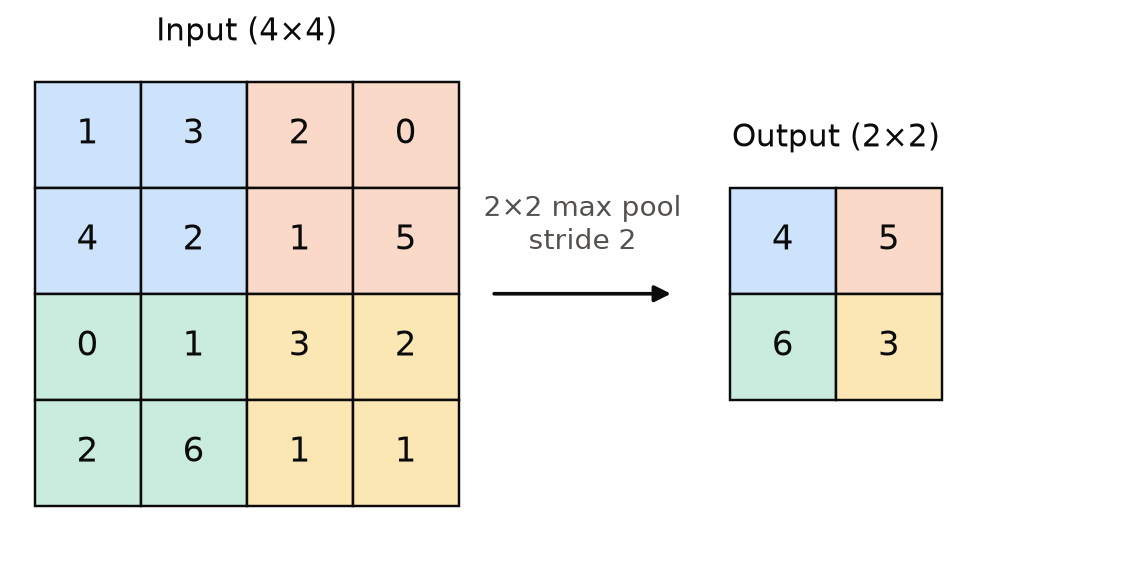
\includegraphics[width=0.48\textwidth]{max_pooling.png}
\caption{$2\times2$ max pooling with stride 2: each coloured window is replaced by its maximum.}
\label{fig:pool}
\end{figure}

\subsection{5. Fully connected layers and the classification head}
After the feature extractor, the feature maps are turned into a vector -- by flattening or by global pooling -- and
passed to one or more fully connected (dense) layers, $\symbf h=\phi(W\symbf x+\symbf b)$, where $\phi$ is ReLU in
hidden layers and softmax in the output layer. Fully connected layers combine evidence from the whole image to make
the final decision. Flattening keeps the spatial layout but is expensive: in our simple CNN, flattening a
$14\times14\times128$ tensor gives 25{,}088 values, and the following 256-unit dense layer alone holds 6.4 million
weights, 96\% of the model. With GAP, as in the complex CNN, the corresponding layer has only 131 thousand weights.

\subsection{6. Training a CNN}
\textbf{Loss function.} A classification CNN is trained by minimizing the cross-entropy between the predicted
distribution and the true label. When the classes are imbalanced, each sample can be weighted by a class weight
$w_{y_i}$ so that errors on rare classes cost more \cite{he2009}:
\begin{equation}
  \mathcal L(\theta) = -\frac{1}{N}\sum_{i=1}^{N} w_{y_i}\,\log \hat y_{i,y_i},
  \label{eq:ce}
\end{equation}
where $\hat y_{i,y_i}$ is the predicted probability of the true class of sample $i$. With all $w_c=1$ this is the
ordinary cross-entropy; Part~2 uses $w_c=N/(K\,n_c)$, where $n_c$ is the number of training images of class $c$.

\textbf{Backpropagation and optimization.} The gradient of the loss with respect to every weight is computed by
backpropagation \cite{rumelhart1986}, i.e.\ the chain rule applied layer by layer from the output back to the input.
The parameters are updated by mini-batch stochastic gradient descent, $\theta\leftarrow\theta-\eta\nabla_\theta
\mathcal L$, where the gradient is estimated on a small batch of images and $\eta$ is the learning rate. We use
\textbf{Adam} \cite{kingma2015}, which keeps exponential moving averages of the gradient $g_t$ and of its square and
gives every parameter its own adaptive step size:
\begin{equation}
  m_t=\beta_1m_{t-1}+(1-\beta_1)g_t,\qquad v_t=\beta_2v_{t-1}+(1-\beta_2)g_t^2,\qquad
  \theta_t=\theta_{t-1}-\eta\frac{\hat m_t}{\sqrt{\hat v_t}+\epsilon}-\eta\lambda\theta_{t-1},
  \label{eq:adam}
\end{equation}
where $\hat m_t,\hat v_t$ are the bias-corrected moments and, by default, $\beta_1=0.9$, $\beta_2=0.999$. The last
term is \textbf{decoupled weight decay} (AdamW) \cite{loshchilov2019}: it shrinks the weights towards zero
independently of the adaptive step and acts as a regularizer. We use $\lambda=10^{-4}$ for the complex CNN and for
fine-tuning ResNet50.

\textbf{Learning-rate schedule, early stopping and mixed precision.} \emph{ReduceLROnPlateau} halves the learning
rate when the monitored validation metric has not improved for a few epochs, so the optimizer takes large steps
early and small steps later. \emph{Early stopping} ends training when the validation metric stops improving and keeps
the best checkpoint, which limits over-fitting and saves time. \emph{Mixed-precision training}
\cite{micikevicius2018} performs most computations in 16-bit floating point while keeping 32-bit master weights (and,
in our models, a 32-bit output layer) for numerical stability; it roughly halves the memory use and speeds up
training on modern GPUs.

\subsection{7. Regularization}
CNNs have millions of parameters and can easily memorize a training set. The following techniques reduce
over-fitting and make training more stable.

\textbf{Dropout.} During training, dropout \cite{srivastava2014} sets each unit of a layer to zero with probability
$p$ and rescales the remaining units, $\tilde{\symbf h}=\frac{1}{1-p}\,\symbf r\odot\symbf h$ with
$r_j\sim\mathrm{Bernoulli}(1-p)$. Because no unit can rely on any particular other unit, the network learns more
robust features and in effect trains an ensemble of thinned sub-networks. Dropout is switched off at test time. Our
models apply dropout with $p$ between 0.3 and 0.5 before their dense layers.

\textbf{Batch normalization.} Batch normalization (BN) \cite{ioffe2015} normalizes every channel with the mean
$\mu_B$ and variance $\sigma_B^2$ of the current mini-batch (computed over the batch and all spatial positions), then
applies a learned scale $\gamma$ and shift $\beta$:
\begin{equation}
  \hat x=\frac{x-\mu_B}{\sqrt{\sigma_B^2+\epsilon}},\qquad y=\gamma\,\hat x+\beta .
  \label{eq:bn}
\end{equation}
At inference time, running averages of $\mu_B$ and $\sigma_B^2$ collected during training are used instead. BN
stabilizes and accelerates training, allows higher learning rates and has a mild regularizing effect. It is part of
almost every modern CNN block; in our complex CNN every convolution is followed by BN.

\textbf{Data augmentation.} Data augmentation enlarges the training set with \emph{label-preserving}
transformations -- flips, crops, zooms, rotations, colour changes -- so that the model sees a slightly different
version of each image in every epoch \cite{shorten2019}. A transformation is only valid if it does not change the
class of the image. As explained in Part~2, this rules out brightness and colour changes in our task, because
brightness and colour are exactly what separates day from dusk and night.

\subsection{8. Classic architectures and CNN blocks}
Progress in CNNs has largely been progress in their building blocks (Table~\ref{tab:archs}):
\begin{itemize}
  \item \textbf{LeNet-5} \cite{lecun1998} stacks two convolution--pooling stages (5$\times$5 kernels, sigmoid,
        average pooling) and three fully connected layers to read handwritten digits; it established the
        conv--pool--FC pattern followed by our simple CNN.
  \item \textbf{AlexNet} \cite{krizhevsky2012} is a deeper and wider LeNet (5 convolutions and 3 dense layers)
        trained on GPUs with ReLU, max pooling, dropout and data augmentation; it won ILSVRC 2012 by a large margin
        and started the deep-learning era in computer vision.
  \item \textbf{VGG} \cite{simonyan2015} showed that depth matters and introduced the \emph{block}: a repeated unit of
        several $3\times3$ convolutions followed by max pooling, doubling the channels after each block. Two stacked
        $3\times3$ convolutions cover a $5\times5$ region with fewer parameters ($18C^2$ vs $25C^2$) and one more
        non-linearity than a single $5\times5$ convolution.
  \item \textbf{NiN} \cite{lin2014} adds $1\times1$ convolutions inside each block and replaces the fully connected
        head by global average pooling, which removes most of the parameters.
  \item \textbf{GoogLeNet} \cite{szegedy2015} is built from Inception blocks, which run $1\times1$, $3\times3$ and
        $5\times5$ convolutions and pooling in parallel and concatenate the results, using $1\times1$ convolutions
        to keep the cost low; it ends with global average pooling instead of large dense layers.
  \item \textbf{ResNet} \cite{he2016} introduced residual blocks with shortcut connections, which made networks with
        50, 101 or even 152 layers trainable; \textbf{DenseNet} \cite{huang2017} concatenates the outputs of all
        previous layers instead of adding them.
\end{itemize}

\begin{table}[htbp]
\centering\small
\caption{Landmark CNN architectures for ImageNet classification.}
\label{tab:archs}
\begin{tabular}{lcccl}
\toprule
Architecture & Year & Weight layers & Parameters & Main idea \\
\midrule
LeNet-5   & 1998 & 5  & $\approx$ 60 K   & conv -- pool -- FC pattern \\
AlexNet   & 2012 & 8  & $\approx$ 60 M   & ReLU, dropout, GPU training \\
VGG-16    & 2015 & 16 & $\approx$ 138 M  & blocks of stacked $3\times3$ convolutions \\
GoogLeNet & 2015 & 22 & $\approx$ 7 M    & Inception blocks, $1\times1$ convolutions, GAP \\
ResNet-50 & 2016 & 50 & $\approx$ 25.6 M & residual (bottleneck) blocks \\
\bottomrule
\end{tabular}
\end{table}

\textbf{Residual learning.} Simply adding layers makes a plain network harder to optimize: beyond some depth even
the training error increases (the \emph{degradation} problem). He et al.\ \cite{he2016} let a block learn a residual
function $\mathcal F(\symbf x)$ and add the input back through a shortcut connection (Figure~\ref{fig:residual}):
\begin{equation}
  \symbf y=\mathcal F(\symbf x)+W_s\symbf x ,
  \label{eq:res}
\end{equation}
where $W_s$ is the identity or, when a block changes the number of channels or the resolution, a $1\times1$
convolution (projection). If the identity mapping is close to optimal, the block only has to push $\mathcal F$
towards zero, which is much easier than learning an identity with a stack of non-linear layers; the shortcut also
gives the gradient a direct path to earlier layers ($\partial\symbf y/\partial\symbf x=\partial\mathcal F/\partial
\symbf x+I$). ResNet-50 uses \emph{bottleneck} blocks in which a $1\times1$ convolution reduces the channels, a
$3\times3$ convolution processes them and another $1\times1$ convolution expands them again (for example
$256\rightarrow64\rightarrow64\rightarrow256$). The ConvBlock of our complex CNN is a simplified residual block with a
projection shortcut.

\begin{figure}[htbp]
\centering
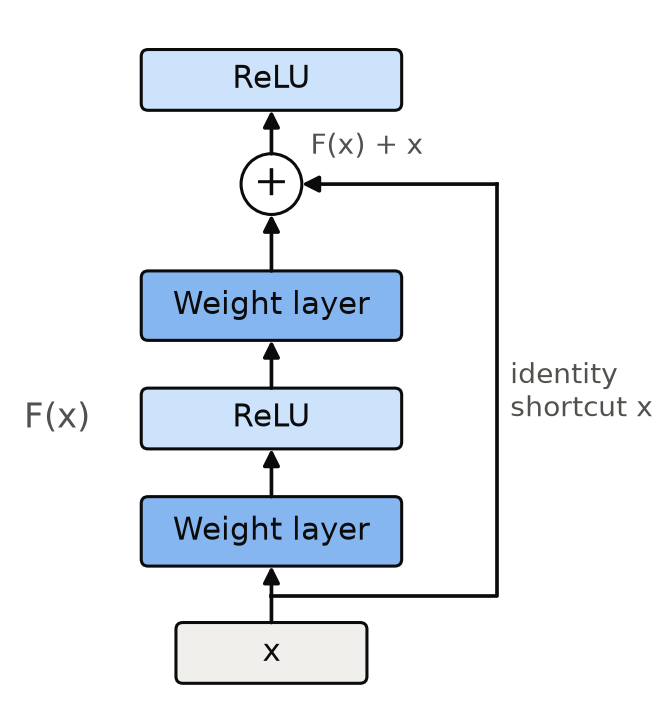
\includegraphics[width=0.3\textwidth]{residual_block.png}
\caption{A residual block: the stacked layers learn $\mathcal F(x)$ and the identity shortcut adds $x$ back before the
final activation.}
\label{fig:residual}
\end{figure}

\subsection{9. Transfer learning and fine-tuning}
Training a deep CNN from scratch requires a large labelled dataset and a lot of computation. Transfer learning reuses
a network already trained on a large source dataset -- usually ImageNet, with 1.28 million images in 1{,}000 classes
\cite{deng2009} -- for a new target task. The early layers of such a network learn generic features (edges, colours,
textures) that transfer well between tasks, while the last layers are more specific to the source task
\cite{yosinski2014}. There are two common strategies:
\begin{itemize}
  \item \textbf{Feature extraction:} freeze the pretrained convolutional base and train only a new classification head
        on top of it. It is fast and works well when the target data are small or similar to the source data.
  \item \textbf{Fine-tuning:} unfreeze part or all of the base and continue training it together with the head, with a
        small learning rate, so that the pretrained features are adapted rather than destroyed.
\end{itemize}
In practice the two are combined in two stages: first the randomly initialized head is trained with the base frozen,
so that large gradients from the untrained head do not damage the pretrained weights; then the base is unfrozen and
the whole network is fine-tuned with a learning rate about ten times smaller. The input must also be preprocessed
exactly as during pretraining. Our third model follows this recipe with ResNet50.

\subsection{10. Evaluation metrics}
For a $K$-class problem, the \textbf{confusion matrix} counts how many test images of true class $i$ are predicted as
class $j$. For each class $k$ we count true positives $TP_k$, false positives $FP_k$ and false negatives $FN_k$, and
define
\begin{equation}
  \begin{gathered}
  \mathrm{Accuracy}=\frac{1}{N}\sum_{i=1}^{N}\symbf 1[\hat y_i=y_i],\qquad
  P_k=\frac{TP_k}{TP_k+FP_k},\qquad R_k=\frac{TP_k}{TP_k+FN_k},\\
  F1_k=\frac{2P_kR_k}{P_k+R_k},\qquad \mathrm{F1}_{\mathrm{macro}}=\frac{1}{K}\sum_{k=1}^{K}F1_k .
  \end{gathered}
  \label{eq:prf}
\end{equation}
Precision answers ``when the model predicts class $k$, how often is it right?'', recall answers ``how many images of
class $k$ does the model find?'', and F1 is their harmonic mean. Macro-averaged precision and recall are defined in
the same way as macro-F1. \textbf{Macro averaging} gives every class the same weight, whatever its size, which matters
for imbalanced data: in our test set the two dawn/dusk classes make up only 8.1\% of the images, so a model that never
predicts them can still have a high accuracy, but its macro-F1 drops sharply. We therefore report accuracy together
with macro precision, recall and F1, select checkpoints by validation macro-F1 and inspect confusion matrices.

\FloatBarrier
% ================================================================================================ PART 2
\newpage
\section{PART 2: PRACTICAL APPLICATION}

\subsection{I. Problem Description}
\subsubsection{1. Title}
\textbf{Time-of-day and weather classification of dashcam images on the BDD100K dataset using convolutional neural
networks.}

\subsubsection{2. Motivation and research objectives}
Lighting and weather are among the main factors that change how a road scene looks to a camera. Perception systems of
autonomous vehicles and advanced driver-assistance systems (ADAS) perform worse at night, at dawn or dusk, and in
rain, fog or snow. Knowing the current condition lets a vehicle adapt -- for example by switching to a detector
trained on night images, increasing safety margins or warning the driver -- and scene-condition labels are useful for
organizing large driving datasets and for testing whether a model is robust across conditions \cite{yu2020}. Weather
recognition from a single image has been studied as a classification problem since early work such as
\cite{lu2014}; we approach it with CNNs on a large real-world driving dataset. The objectives of the project are:
\begin{itemize}
  \item to build a six-class image classification task from the time-of-day and weather attributes of BDD100K and
        prepare the data (cleaning, label merging, splitting, resizing, normalization and augmentation);
  \item to design and train three CNNs of increasing capacity: a simple CNN made of convolution, pooling and fully
        connected layers; a more complex CNN made of residual CNN blocks with batch normalization; and a transfer
        learning model that fine-tunes ResNet50 pretrained on ImageNet;
  \item to evaluate and compare the models on a held-out test set with accuracy, macro precision, recall and F1-score
        and confusion matrices, measure the effect of data augmentation and analyse the typical errors.
\end{itemize}

\subsubsection{3. Input and output of the problem}
\begin{itemize}
  \item \textbf{Input:} one RGB image taken by the front dashcam of a car. Original images are $1280\times720$
        pixels; they are resized to $224\times224\times3$ and normalized before entering the network.
  \item \textbf{Output:} one of six classes that combine the time of day and the weather (Table~\ref{tab:classes}).
        The network outputs a probability vector $\hat{\symbf y}\in[0,1]^6$ through a softmax layer, and the
        predicted class is the one with the highest probability.
\end{itemize}

\begin{table}[htbp]
\centering\small
\caption{The six target classes (class index in brackets).}
\label{tab:classes}
\begin{tabular}{lll}
\toprule
Time of day & Clear (clear, partly cloudy) & Unclear (overcast, rainy, snowy, foggy) \\
\midrule
Daytime   & daytime\_clear (0)  & daytime\_unclear (1)  \\
Night     & night\_clear (2)    & night\_unclear (3)    \\
Dawn/dusk & dawndusk\_clear (4) & dawndusk\_unclear (5) \\
\bottomrule
\end{tabular}
\end{table}

\subsubsection{4. Summary of the tasks performed}
\begin{enumerate}[leftmargin=1.6em]
  \item Downloaded BDD100K from Kaggle and read the image-level time-of-day and weather labels of the official
        training and validation sets.
  \item Merged the labels into six classes, removed images with undefined attributes, checked that every image could
        be decoded and that no image appears in two subsets.
  \item Split the data into training, validation and test sets (the official validation set serves as the test set)
        and resized all images to $224\times224$ pixels.
  \item Built one data pipeline for all models: ImageNet normalization, label-preserving augmentation (horizontal flip
        and small zoom), class-weighted loss, checkpoint selection by validation macro-F1, early stopping and
        learning-rate reduction.
  \item Designed and trained Model~1 (simple CNN), Model~2 (complex CNN built from residual ConvBlocks) and Model~3
        (ResNet50 transfer learning in two stages); Model~1 was also trained without augmentation as an ablation.
  \item Evaluated all models on the test set and analysed per-class results, confusion matrices and misclassified
        images.
\end{enumerate}
The workflow is summarized in Figure~\ref{fig:pipeline}. The code is written in Python with Keras~3
\cite{chollet2015} running on the PyTorch backend \cite{paszke2019} and scikit-learn \cite{pedregosa2011}; it is
available in the project repository \cite{repo}, where the scripts are numbered in the order they are run
(\texttt{01\_prepare\_data.py} to \texttt{07\_compare.py}).

\begin{figure}[htbp]
\centering
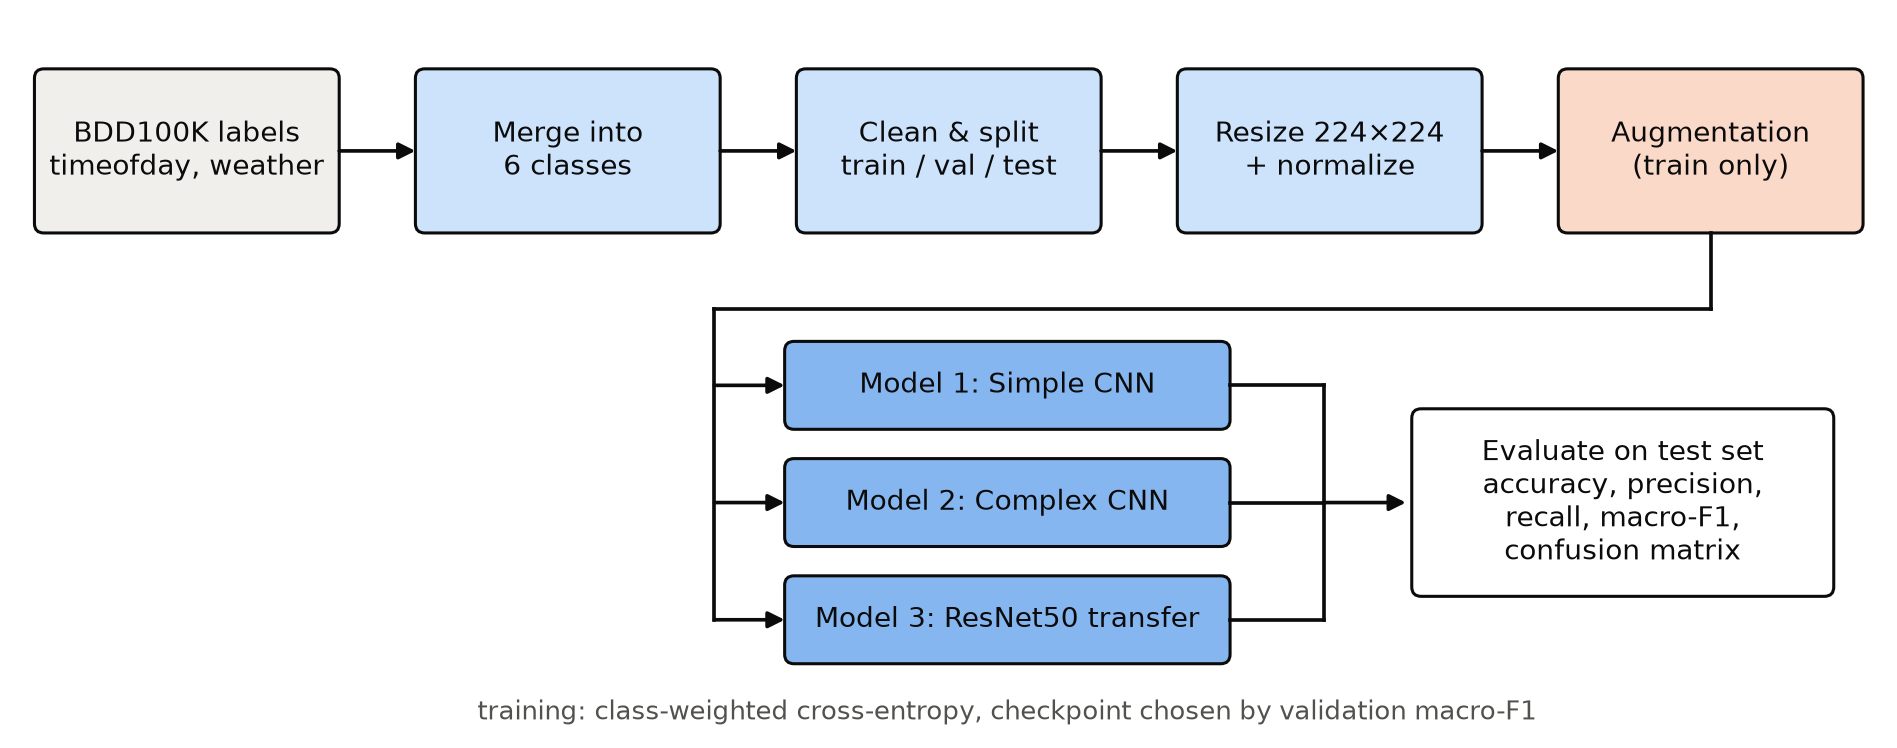
\includegraphics[width=0.86\textwidth]{pipeline.png}
\caption{Workflow of the project.}
\label{fig:pipeline}
\end{figure}

\subsection{II. Dataset Description}
\subsubsection{1. Download link}
We use \textbf{BDD100K} (Berkeley DeepDrive 100K), a large and diverse driving dataset released by UC Berkeley
\cite{yu2020}:
\begin{itemize}
  \item Kaggle mirror used in this project \cite{kaggle}:
        \url{https://www.kaggle.com/datasets/solesensei/solesensei_bdd100k}
  \item Official website \cite{bddsite}: \url{https://bdd-data.berkeley.edu}
\end{itemize}

\subsubsection{2. Description of the dataset}
BDD100K consists of 100{,}000 driving videos of about 40 seconds each, recorded at 720p by dashcams in more than
50{,}000 rides, mainly in New York and the San Francisco Bay Area \cite{yu2020}. One keyframe of every video is
annotated, giving \textbf{100{,}000 images of $1280\times720$ pixels} (RGB, JPEG), split into 70{,}000 training,
10{,}000 validation and 20{,}000 test images. The annotations include image-level attributes (weather, scene type and
time of day, Table~\ref{tab:attrs}); bounding boxes of 10 object categories (car, bus, truck, train, person, rider,
bike, motorcycle, traffic light and traffic sign); drivable areas and lane markings; and pixel-level semantic and
instance segmentation for a subset of 10{,}000 images. The images therefore show ordinary road scenes -- vehicles,
pedestrians, cyclists, traffic lights and signs, buildings, road and sky -- under a wide range of lighting and weather
conditions. In this project only the \textbf{time of day} and \textbf{weather} attributes are used. Labels of the
20{,}000 official test images are not public, so we work with the official training set (its label file contains
69{,}863 images) and the official validation set (10{,}000 images).

\begin{table}[htbp]
\centering\small
\caption{Image-level attributes of BDD100K.}
\label{tab:attrs}
\begin{tabular}{ll}
\toprule
Attribute & Possible values \\
\midrule
weather   & clear, partly cloudy, overcast, rainy, snowy, foggy, undefined \\
scene     & city street, highway, residential, parking lot, gas stations, tunnel, undefined \\
timeofday & daytime, night, dawn/dusk, undefined \\
\bottomrule
\end{tabular}
\end{table}

\subsubsection{3. Label definition}
The time of day is kept as it is and images marked \emph{undefined} are removed. The weather is merged into two groups:
\emph{clear} and \emph{partly cloudy} become \textbf{clear}, while \emph{overcast}, \emph{rainy}, \emph{snowy} and
\emph{foggy} become \textbf{unclear}; images marked \emph{undefined} are removed. A partly cloudy sky still gives a
clear view and normal lighting, whereas overcast skies, rain, snow and fog all reduce visibility and contrast.
Keeping the six weather values separately would create many tiny classes -- foggy images, for example, number only
143 in the whole dataset and 16 at dawn/dusk (Table~\ref{tab:attrcounts}) -- which could not be learned or evaluated
reliably. Table~\ref{tab:attrcounts} also shows a property of the labels that matters later: almost no night image is
tagged overcast or partly cloudy (144 of 31{,}392), because the sky cannot be seen in the dark.

\begin{table}[htbp]
\centering\small
\caption{Original time-of-day and weather tags of the 70{,}569 images kept (training + validation + test).}
\label{tab:attrcounts}
\begin{tabular}{lrrrrrrr}
\toprule
timeofday & clear & partly cloudy & overcast & rainy & snowy & foggy & total \\
\midrule
dawn/dusk & 2{,}311  & 665     & 1{,}329  & 383     & 510     & 16  & 5{,}214 \\
daytime   & 14{,}218 & 4{,}900 & 8{,}590  & 2{,}918 & 3{,}284 & 53  & 33{,}963 \\
night     & 26{,}158 & 54      & 90       & 2{,}494 & 2{,}522 & 74  & 31{,}392 \\
\midrule
\textbf{total} & \textbf{42{,}687} & \textbf{5{,}619} & \textbf{10{,}009} & \textbf{5{,}795} & \textbf{6{,}316}
  & \textbf{143} & \textbf{70{,}569} \\
\bottomrule
\end{tabular}
\end{table}

\subsubsection{4. Number of images and class distribution}
After cleaning, \textbf{70{,}569 images} remain. Table~\ref{tab:counts} gives the number of images per class and
subset, and Figure~\ref{fig:dist} shows the overall distribution. The classes are clearly \textbf{imbalanced}:
night\_clear has 26{,}212 images (37.1\%) while dawndusk\_unclear has only 2{,}238 (3.2\%), a ratio of about 12 to 1.
Dawn and dusk are short periods of the day, so they are naturally rare in driving data, and the two dawn/dusk classes
together account for only 7.4\% of the images. Because the split is stratified and the official validation set
follows a similar distribution, the three subsets have almost the same class proportions. The imbalance is handled
with class weights and macro-F1 model selection (Section III).

\begin{table}[htbp]
\centering\small
\caption{Number of images per class in each subset.}
\label{tab:counts}
\begin{tabular}{lrrrrr}
\toprule
Class & Train & Validation & Test & Total & Share \\
\midrule
daytime\_clear    & 13{,}373 & 3{,}343 & 2{,}402 & 19{,}118 & 27.1\% \\
daytime\_unclear  & 10{,}386 & 2{,}597 & 1{,}862 & 14{,}845 & 21.0\% \\
night\_clear      & 18{,}346 & 4{,}587 & 3{,}279 & 26{,}212 & 37.1\% \\
night\_unclear    &  3{,}677 &   919   &   584   &  5{,}180 &  7.3\% \\
dawndusk\_clear   &  2{,}059 &   515   &   402   &  2{,}976 &  4.2\% \\
dawndusk\_unclear &  1{,}541 &   385   &   312   &  2{,}238 &  3.2\% \\
\midrule
\textbf{Total}    & \textbf{49{,}382} & \textbf{12{,}346} & \textbf{8{,}841} & \textbf{70{,}569} & 100\% \\
\bottomrule
\end{tabular}
\end{table}

\begin{figure}[htbp]
\centering
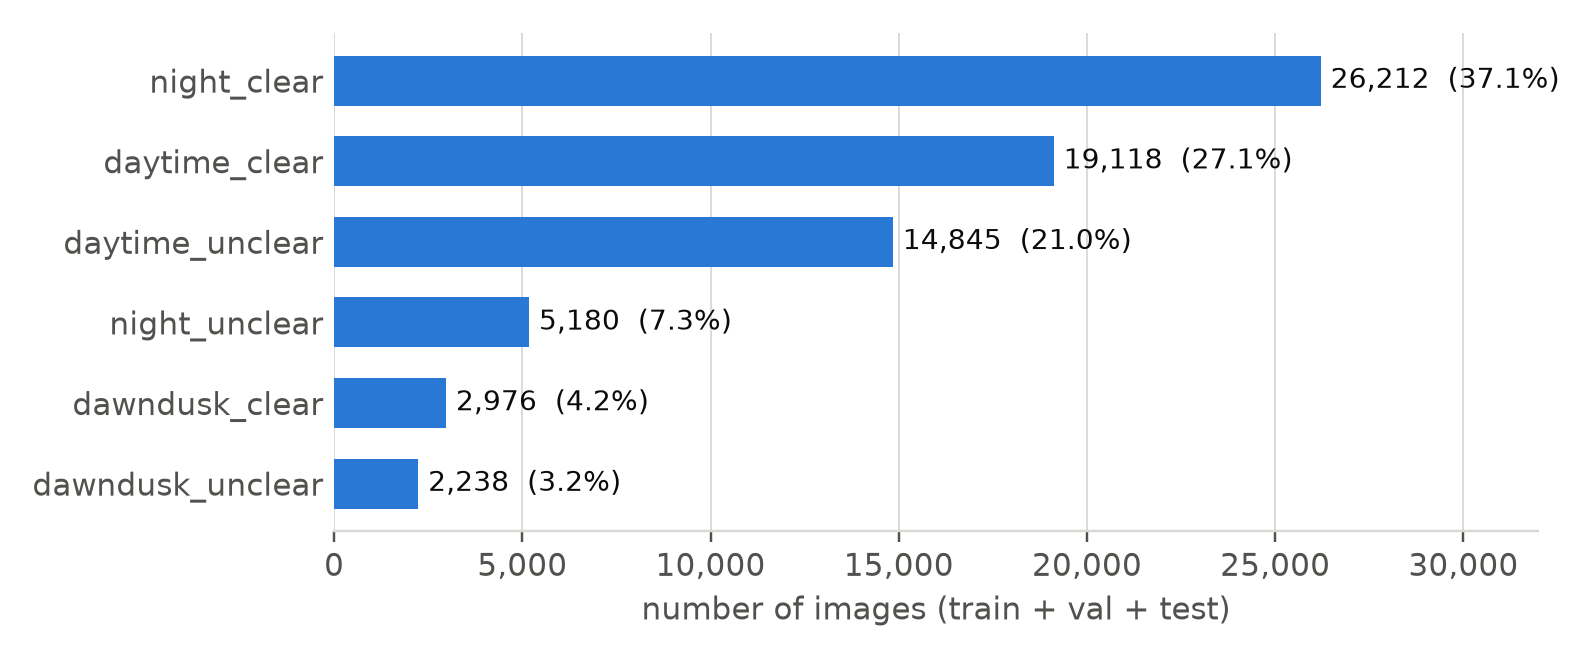
\includegraphics[width=0.6\textwidth]{class_distribution.png}
\caption{Class distribution over the whole dataset.}
\label{fig:dist}
\end{figure}

Figure~\ref{fig:samples} shows random test images of every class. Day and night are easy to tell apart for a human,
but several difficulties are visible: dawn/dusk images range from almost-day to almost-night; \emph{partly cloudy}
(clear) and \emph{overcast} (unclear) skies can look very similar; and rain is often visible only as drops on the
windshield or as a wet, reflective road. The tags were assigned by human annotators from a single frame, so some of
them are ambiguous or noisy.

\begin{figure}[htbp]
\centering
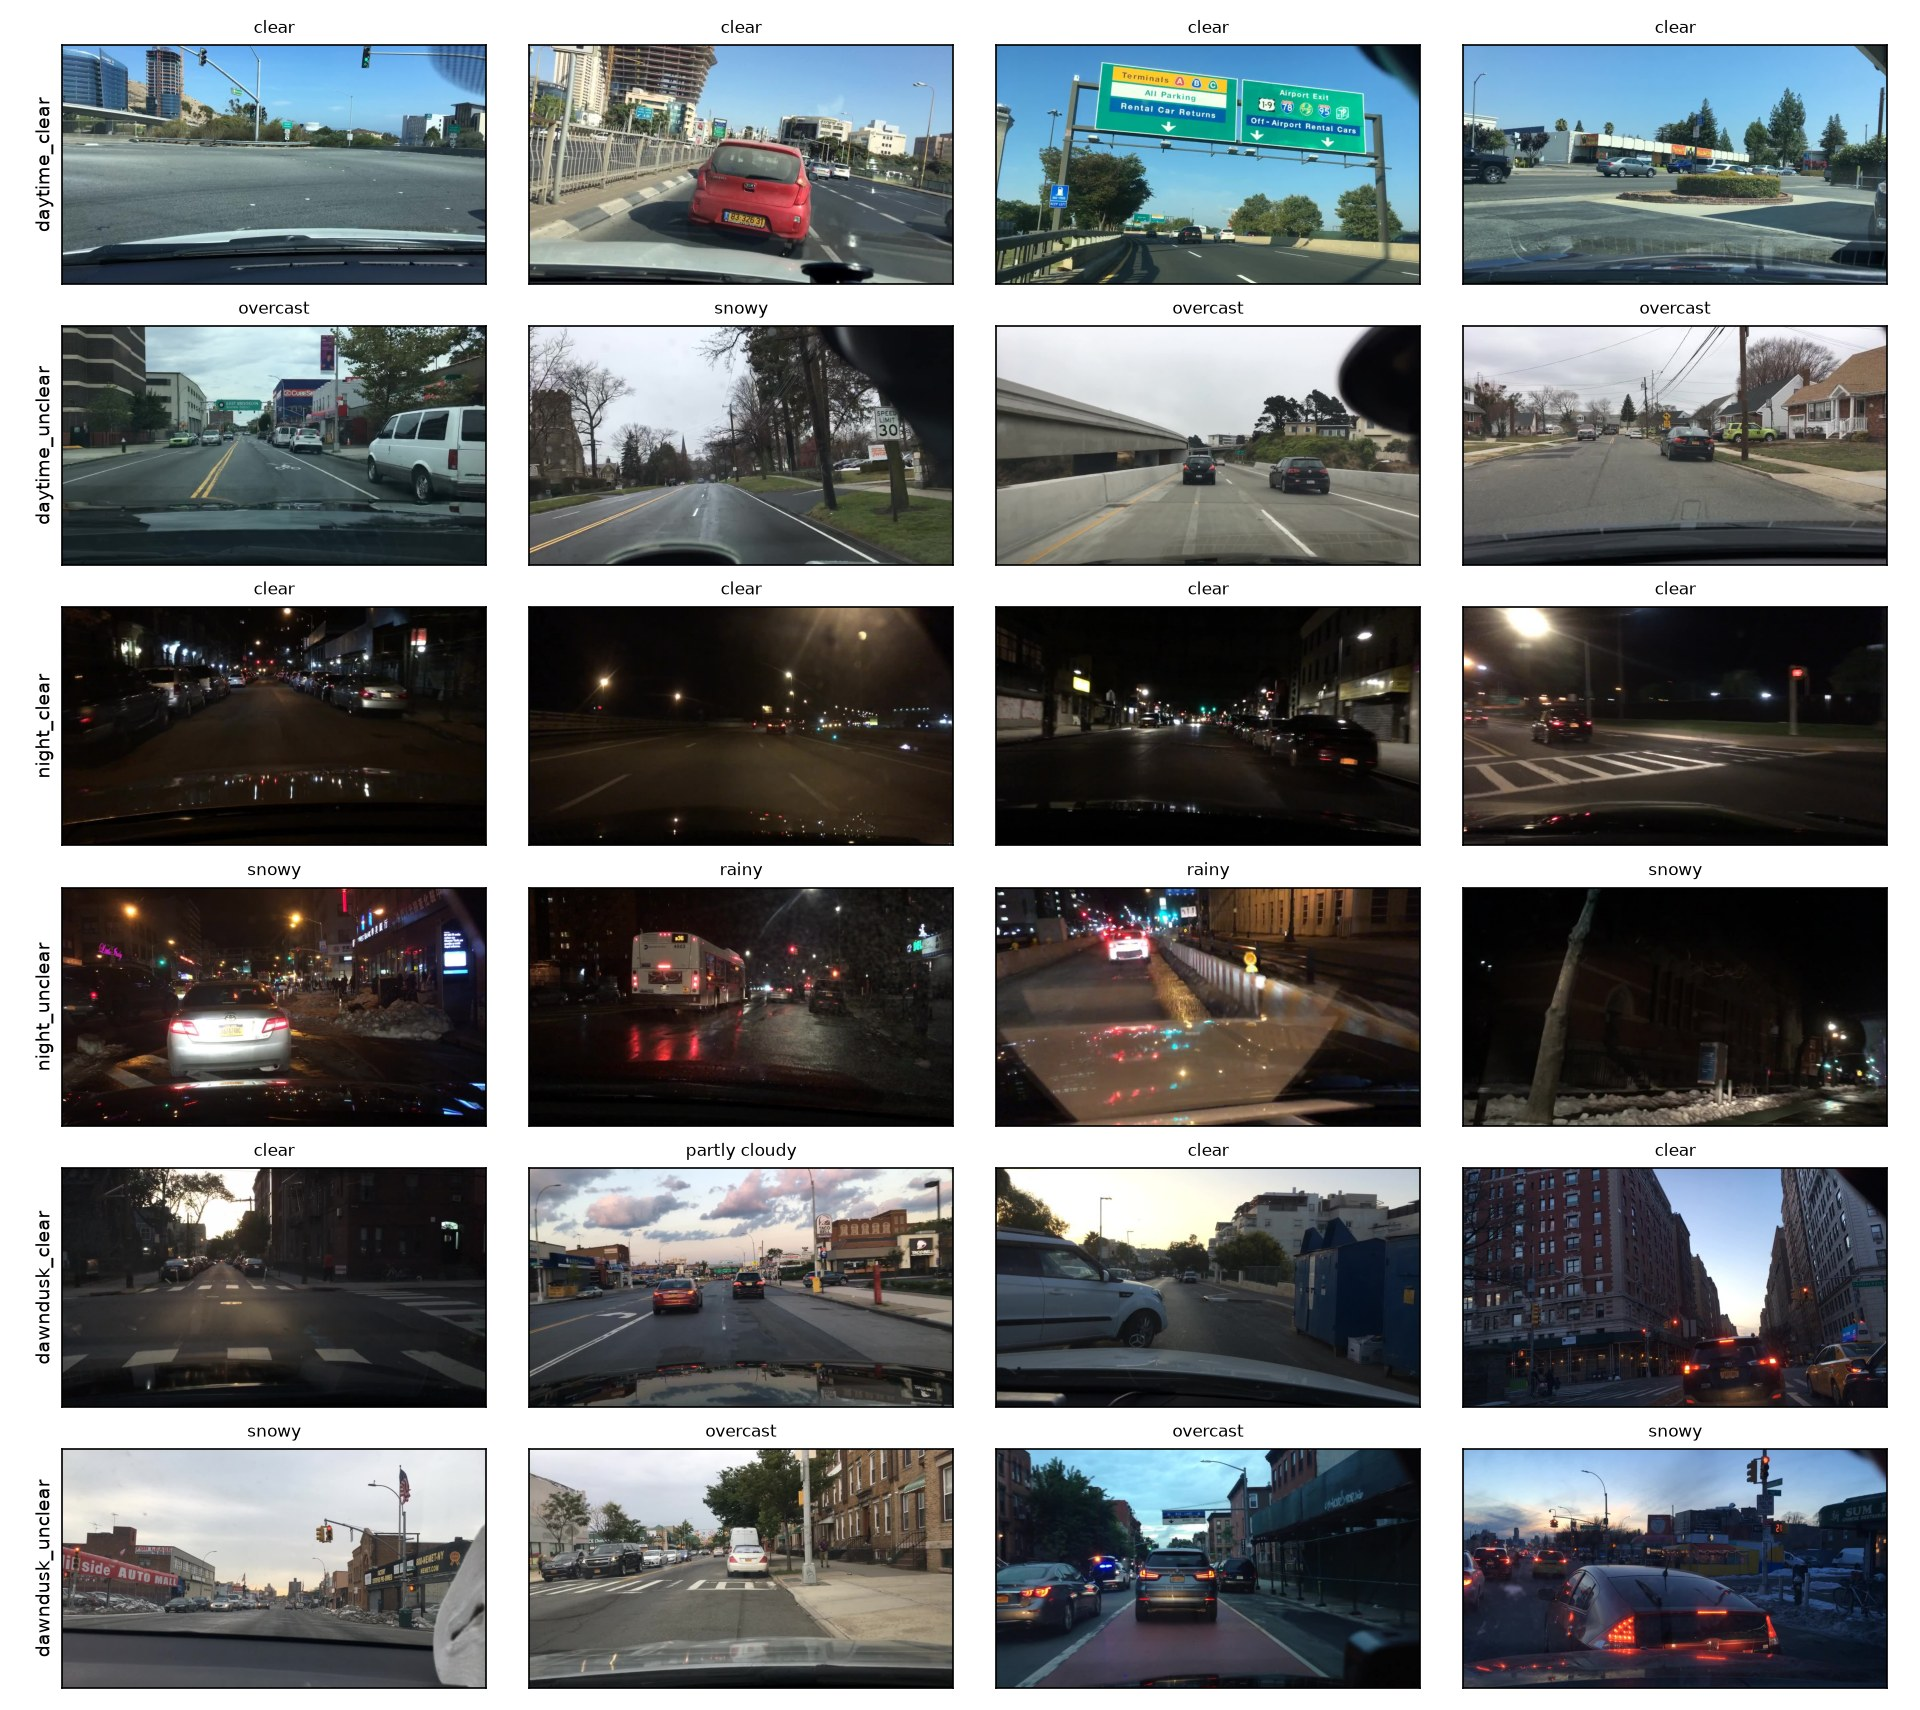
\includegraphics[width=0.6\textwidth]{samples.jpg}
\caption{Random test images of the six classes; the original weather tag is printed above each image.}
\label{fig:samples}
\end{figure}

\subsubsection{5. Image size}
All BDD100K images have the same size: \textbf{$1280\times720$ pixels} (16:9), three colour channels, stored as JPEG.
For training they are resized to $224\times224$ pixels (Section III).

\FloatBarrier
% ------------------------------------------------------------------------------------------------ III
\subsection{III. CNN Model Design}

\subsubsection{1. Data preprocessing}
\textbf{Cleaning.} Images whose time of day or weather is \emph{undefined} were removed: 8{,}135 of the 69{,}863
official training images (11.6\%) and 1{,}159 of the 10{,}000 official validation images. Every remaining image was
opened and decoded; missing or corrupted files would have been skipped and counted, but none were found. Finally,
the preparation script asserts that no file name appears in two subsets, which rules out leakage between the
training, validation and test data.

\textbf{Resizing.} The $1280\times720$ images were resized once, offline, to $224\times224$ pixels and saved as JPEG
(quality 95), which makes loading during training much faster (each image is about 18 times smaller). The aspect
ratio is not preserved; the horizontal squeeze is the same for all images and does not affect global cues such as
brightness, sky colour or haze, and $224\times224$ is the input size for which ResNet50 was pretrained.

\textbf{Normalization.} Pixel values are scaled to $[0,1]$ and standardized per channel with the ImageNet statistics,
$x'=(x/255-\mu)/\sigma$ with $\mu=(0.485,0.456,0.406)$ and $\sigma=(0.229,0.224,0.225)$. The same normalization is
used for the three models so that they share one data pipeline. The Keras ResNet50 weights expect a different
(``Caffe'') preprocessing -- BGR channel order and subtraction of the ImageNet mean on the 0--255 scale -- so Model~3
contains a small layer that converts the standardized input into that format (Section III.6). Images are read batch
by batch by a \texttt{keras.utils.PyDataset} with four reader threads; only the training set is shuffled.

\textbf{Augmentation.} Augmentation is the first block of every model, so it runs on the GPU, only during training,
and is automatically switched off for validation and testing. It consists of a random \textbf{horizontal flip} -- a
mirrored road scene is still a valid road scene with the same time and weather -- and a random \textbf{zoom-in} of up
to 10\% along each axis, i.e.\ a random crop that keeps 90--100\% of the height and of the width, which imitates small
changes of camera position and field of view. We deliberately do \textbf{not} use brightness, contrast, saturation or
hue changes, grey-scale conversion or vertical flips. Brightness and colour are exactly the cues that separate day,
dusk and night, and fog or an overcast sky lower the contrast and saturation of the image; changing them would turn a
daytime image into a dusk-like image, or a clear image into a hazy one, while keeping the old label -- that is, it
would add label noise. A vertical flip puts the sky at the bottom of the image, which never happens in practice.

\textbf{Class imbalance.} So that the models do not ignore the rare dawn/dusk classes, the loss is weighted per class
(Eq.~\ref{eq:ce}) with $w_c=N/(K\,n_c)$ computed on the training set (Table~\ref{tab:weights}). An error on a
dawndusk\_unclear image costs about 12 times more than an error on a night\_clear image, so every class contributes
equally to the loss on average. Because \texttt{fit(class\_weight=...)} is not supported with a \texttt{PyDataset},
each training batch returns the class weight of every image as a sample weight. In addition, the checkpoint kept for
each model is the one with the highest \textbf{macro-F1 on the validation set}, not the highest accuracy.

\begin{table}[htbp]
\centering\small
\caption{Class weights used in the loss function ($N$ = 49{,}382 training images, $K$ = 6).}
\label{tab:weights}
\begin{tabular}{lrr}
\toprule
Class & Training images $n_c$ & Class weight $w_c$ \\
\midrule
daytime\_clear    & 13{,}373 & 0.615 \\
daytime\_unclear  & 10{,}386 & 0.792 \\
night\_clear      & 18{,}346 & 0.449 \\
night\_unclear    &  3{,}677 & 2.238 \\
dawndusk\_clear   &  2{,}059 & 3.997 \\
dawndusk\_unclear &  1{,}541 & 5.341 \\
\bottomrule
\end{tabular}
\end{table}

\subsubsection{2. Data splitting}
Because the official test labels are not available, the official validation set (8{,}841 images after cleaning) is
used as our \textbf{test set}; it is never used for training or model selection. The cleaned official training set
(61{,}728 images) is split 80/20 into a \textbf{training} and a \textbf{validation} set with scikit-learn's
\texttt{train\_test\_split}, stratified by class and with \texttt{random\_state = 42} so that the split is
reproducible (Table~\ref{tab:split}). The training set is used to fit the weights; the validation set is evaluated
after every epoch for early stopping, learning-rate reduction and checkpoint selection; the test set is used once,
at the end, to report the final results.

\begin{table}[htbp]
\centering\small
\caption{The three subsets.}
\label{tab:split}
\begin{tabular}{llrrl}
\toprule
Subset & Source & Images & Share & Purpose \\
\midrule
Training   & 80\% of official train & 49{,}382 & 70.0\% & fit the weights \\
Validation & 20\% of official train & 12{,}346 & 17.5\% & early stopping, LR schedule, checkpoint \\
Test       & official validation    & 8{,}841  & 12.5\% & final evaluation only \\
\midrule
\textbf{Total} & & \textbf{70{,}569} & 100\% & \\
\bottomrule
\end{tabular}
\end{table}

\subsubsection{3. Common training setup}
The three models share the training procedure of Part~1, Section~6 (Table~\ref{tab:setup}). The loss is the
class-weighted cross-entropy and the optimizer is Adam. A callback computes the loss, accuracy and macro-F1 on the
whole validation set after every epoch (macro-F1 cannot be averaged over batches); the learning rate is halved when
the validation macro-F1 does not improve for 2 epochs, training stops early when it does not improve for several
epochs, and the weights of the best epoch are restored for testing. All models were trained on one NVIDIA GeForce
RTX 3060 GPU (12~GB) with Keras~3 on the PyTorch backend (CUDA 12.6), using mixed float16 precision and a fixed
random seed of 42. A second callback frees GPU memory after every batch, which removed random out-of-memory errors at
the start of epochs.

\begin{table}[htbp]
\centering\small
\caption{Training settings of the three models.}
\label{tab:setup}
\begin{tabular}{llll}
\toprule
Setting & Model 1: Simple CNN & Model 2: Complex CNN & Model 3: ResNet50 \\
\midrule
Augmentation           & flip + zoom (and none)  & flip + zoom        & flip + zoom \\
Initial learning rate  & $10^{-3}$               & $3\times10^{-4}$   & $10^{-3}$ / $10^{-4}$ (stage 1 / 2) \\
Weight decay           & --                      & $10^{-4}$          & -- / $10^{-4}$ \\
Batch size             & 64                      & 32                 & 32 \\
Max epochs             & 20                      & 25                 & 3 + 10 \\
Early-stopping patience & 5                      & 5                  & 3 / 3 \\
Trainable parameters   & 6.67 M                  & 5.02 M             & 12.3 K / 23.5 M \\
\bottomrule
\end{tabular}
\end{table}

\subsubsection{4. Model 1 -- Simple CNN}
\begin{figure}[htbp]
\centering
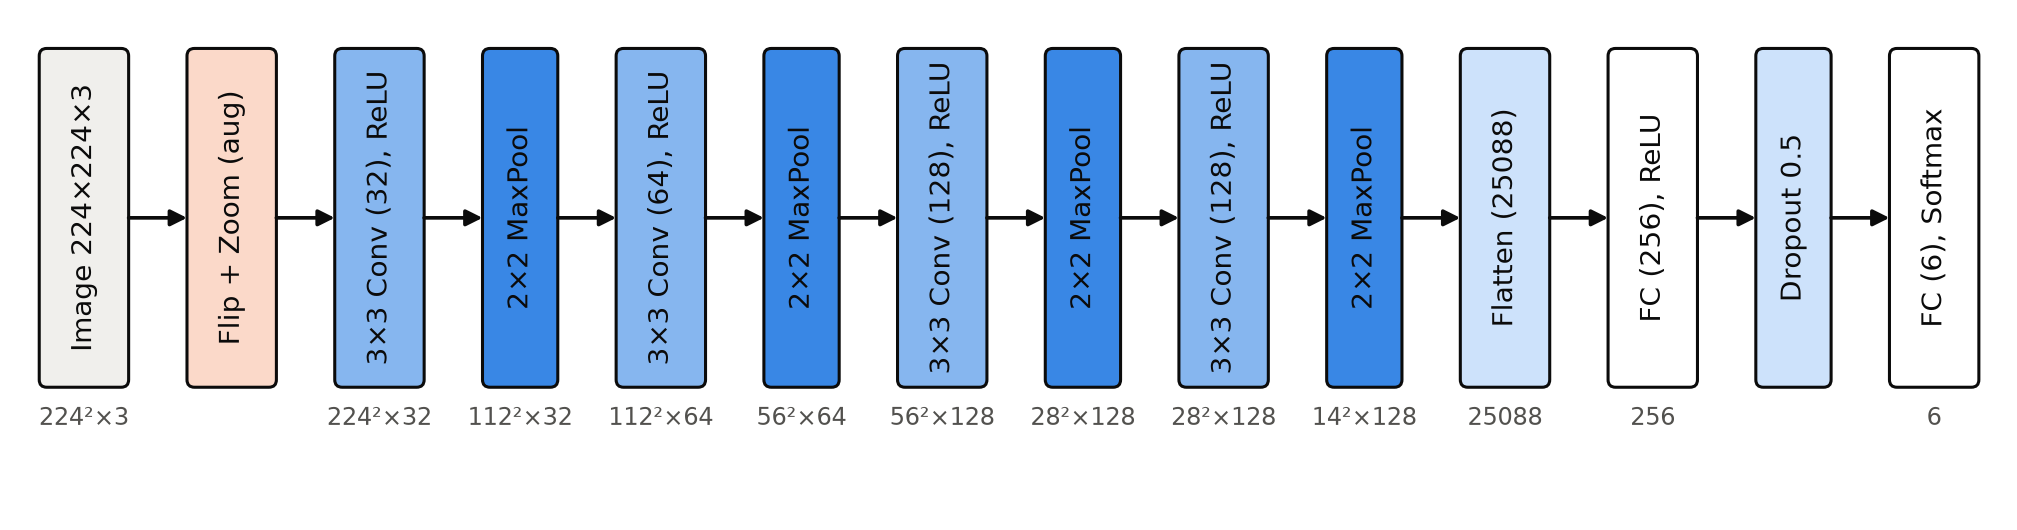
\includegraphics[width=\textwidth]{simple_cnn.png}
\caption{Architecture of Model 1. Numbers under the boxes are output shapes (height$^2\times$channels).}
\label{fig:simple}
\end{figure}

\textbf{Structure.} Four stages of a $3\times3$ convolution (same padding, ReLU) followed by a $2\times2$ max pooling,
with 32, 64, 128 and 128 filters, reduce the image from $224\times224\times3$ to $14\times14\times128$. The feature
maps are flattened into a 25{,}088-dimensional vector and classified by a fully connected layer of 256 ReLU units,
dropout with rate 0.5 and a 6-unit softmax layer (Figure~\ref{fig:simple}). Table~\ref{tab:simple} lists the layers;
the number of parameters is $(k^2C_{in}+1)C_{out}$ for a convolution and $(n_{in}+1)n_{out}$ for a dense layer.

\begin{table}[htbp]
\centering\small
\caption{Layers of Model 1.}
\label{tab:simple}
\begin{tabular}{llr}
\toprule
Layer & Output shape & Parameters \\
\midrule
Input + augmentation (flip, zoom)      & $224\times224\times3$  & 0 \\
Conv $3\times3$, 32 filters, ReLU      & $224\times224\times32$ & 896 \\
MaxPool $2\times2$                     & $112\times112\times32$ & 0 \\
Conv $3\times3$, 64 filters, ReLU      & $112\times112\times64$ & 18{,}496 \\
MaxPool $2\times2$                     & $56\times56\times64$   & 0 \\
Conv $3\times3$, 128 filters, ReLU     & $56\times56\times128$  & 73{,}856 \\
MaxPool $2\times2$                     & $28\times28\times128$  & 0 \\
Conv $3\times3$, 128 filters, ReLU     & $28\times28\times128$  & 147{,}584 \\
MaxPool $2\times2$                     & $14\times14\times128$  & 0 \\
Flatten                                & 25{,}088               & 0 \\
Dense 256, ReLU + Dropout 0.5          & 256                    & 6{,}422{,}784 \\
Dense 6, softmax                       & 6                      & 1{,}542 \\
\midrule
\textbf{Total}                         &                        & \textbf{6{,}665{,}158} \\
\bottomrule
\end{tabular}
\end{table}

\textbf{Why this design.} Model~1 is the baseline required by the assignment and follows the classic LeNet/VGG pattern
conv $\rightarrow$ pool $\rightarrow\dots\rightarrow$ fully connected \cite{lecun1998,simonyan2015}, with $3\times3$
kernels (VGG) instead of LeNet's $5\times5$ ones and ReLU and max pooling instead of sigmoid and average pooling. Four
pooling stages are needed to bring a $224\times224$ image to a small $14\times14$ grid; the number of filters doubles
while the resolution halves, which keeps the computation per stage similar, and is capped at 128 in the last stage to
keep the flattened vector and the first dense layer manageable. Even so, this dense layer holds 96\% of the 6.7~M
parameters, which is why a strong dropout of 0.5 follows it. The model deliberately has no batch normalization, no
shortcuts and no blocks, so that the gain from these components can be measured with Model~2.

\textbf{Ablation without augmentation.} To measure the effect of data augmentation, Model~1 was also trained without
its augmentation block, with everything else unchanged (architecture, seed, optimizer, learning rate and number of
epochs). The two versions are called \emph{Simple CNN} and \emph{Simple CNN + Aug} in Section IV.

\subsubsection{5. Model 2 -- Complex CNN built from residual blocks}
\textbf{Structure.} The network is built from a reusable \textbf{ConvBlock} (Figure~\ref{fig:convblock}): a main
branch with two $3\times3$ convolutions, each followed by BN, with a ReLU between them; a shortcut branch with a
$1\times1$ convolution and BN that projects the input to the same number of channels; the two branches are added,
passed through a ReLU and a $2\times2$ max pooling, so every block doubles the number of channels and halves the
resolution. Because of the two branches the model is written with the Keras functional API instead of
\texttt{Sequential}. The full model (Figure~\ref{fig:complex}, Table~\ref{tab:complex}) is a stride-2 stem
convolution (32 filters, BN, ReLU), four ConvBlocks with 64, 128, 256 and 512 channels, global average pooling and a
head of dropout 0.3, a 256-unit dense layer, dropout 0.3 and the softmax.

\begin{figure}[htbp]
\centering
\begin{minipage}[c]{0.36\textwidth}
  \centering
  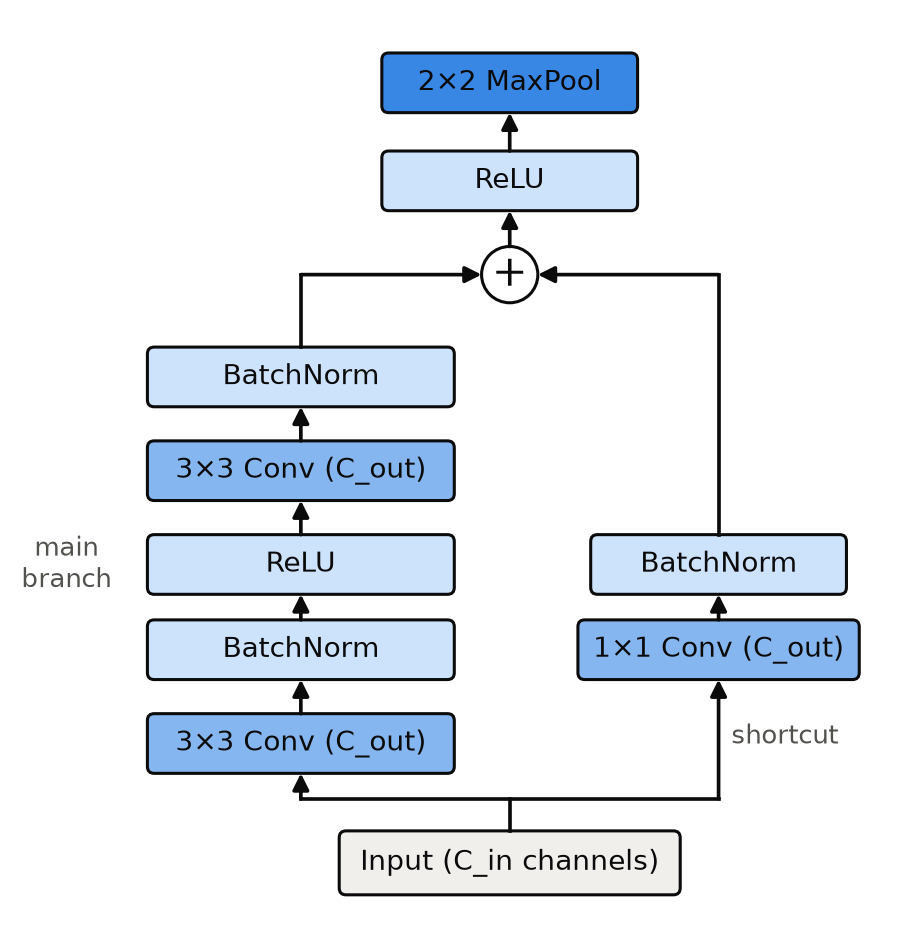
\includegraphics[width=\textwidth]{conv_block.png}
  \caption{The ConvBlock of Model 2.}
  \label{fig:convblock}
\end{minipage}\hfill
\begin{minipage}[c]{0.6\textwidth}
  \centering\small
  \captionof{table}{Stages of Model 2 (a BN layer has 4 parameters per channel: $\gamma,\beta$ and the running mean
  and variance).}
  \label{tab:complex}
  \begin{tabular}{llr}
  \toprule
  Stage & Output & Parameters \\
  \midrule
  Stem conv /2 + BN       & $112^2\times32$ & 1{,}024 \\
  ConvBlock 1 (32$\rightarrow$64)   & $56^2\times64$  & 58{,}304 \\
  ConvBlock 2 (64$\rightarrow$128)  & $28^2\times128$ & 231{,}296 \\
  ConvBlock 3 (128$\rightarrow$256) & $14^2\times256$ & 921{,}344 \\
  ConvBlock 4 (256$\rightarrow$512) & $7^2\times512$  & 3{,}677{,}696 \\
  GAP                     & 512             & 0 \\
  Dense 256 + dropouts    & 256             & 131{,}328 \\
  Dense 6, softmax        & 6               & 1{,}542 \\
  \midrule
  \textbf{Total}          &                 & \textbf{5{,}022{,}534} \\
  \bottomrule
  \end{tabular}
\end{minipage}
\end{figure}

\begin{figure}[htbp]
\centering
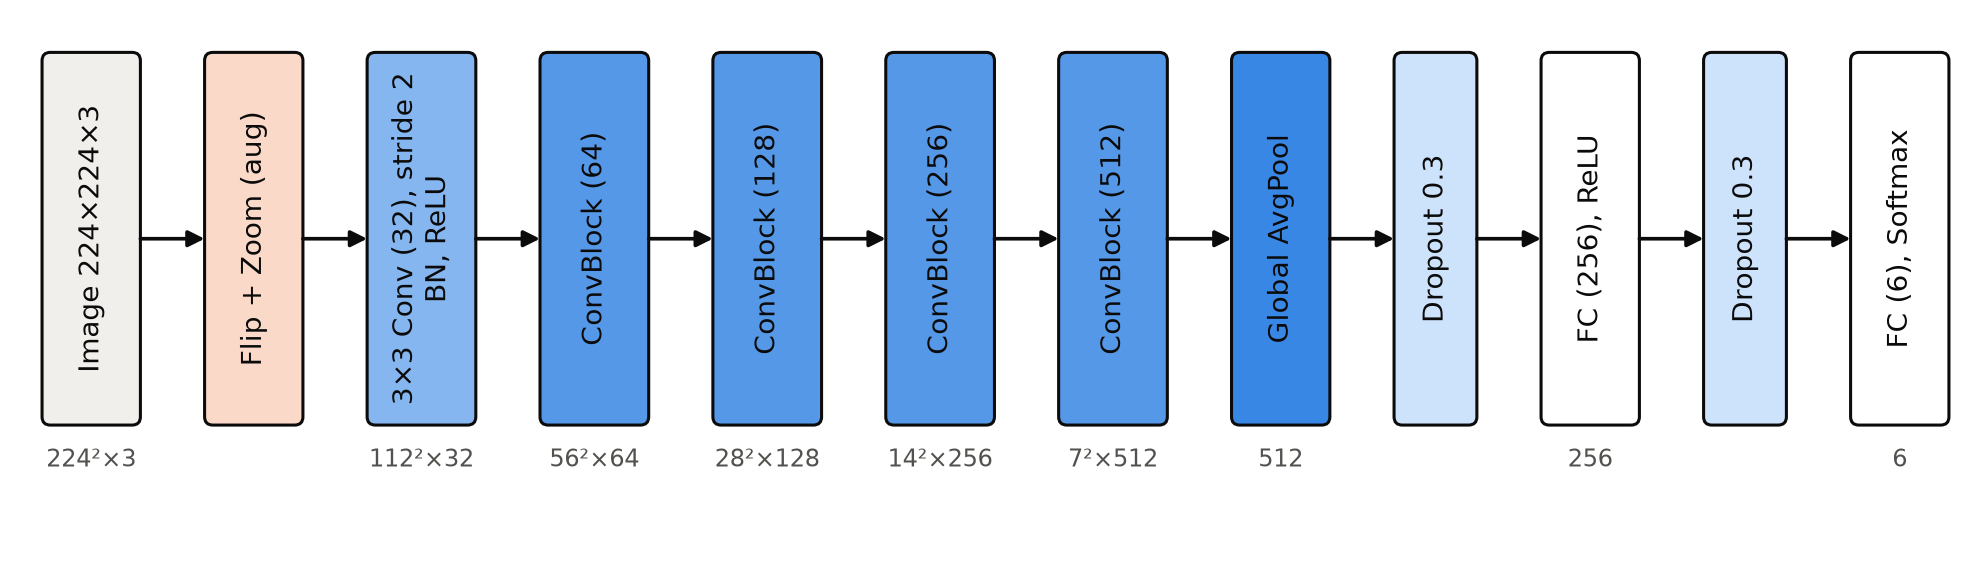
\includegraphics[width=\textwidth]{complex_cnn.png}
\caption{Architecture of Model 2. Numbers under the boxes are output shapes.}
\label{fig:complex}
\end{figure}

As an example of the parameter count, ConvBlock~1 has $(9\cdot32+1)\cdot64=18{,}496$ and $(9\cdot64+1)\cdot64=36{,}928$
parameters in its two $3\times3$ convolutions, $(32+1)\cdot64=2{,}112$ in the $1\times1$ shortcut and $3\cdot4\cdot64=768$
in its three BN layers, 58{,}304 in total; of the 5{,}022{,}534 parameters of the model, 5{,}824 are BN running
statistics that are not trained by gradient descent.

\textbf{Why this design.} Each choice addresses a weakness of Model~1:
\begin{itemize}
  \item \emph{Two $3\times3$ convolutions per block} (VGG) double the depth at each resolution and enlarge the
        receptive field cheaply, so the network can combine more local evidence (raindrops, wet road, snow patches)
        before pooling.
  \item \emph{Batch normalization} after every convolution stabilizes the training of the deeper network.
  \item \emph{Residual shortcuts} (ResNet) keep the deeper network easy to optimize; a $1\times1$ projection is needed
        because every block changes the number of channels.
  \item \emph{Global average pooling instead of flattening} removes the huge dense layer of Model~1 (the head now has
        only 133~K parameters) and matches the nature of the task: time of day and weather are \emph{global}
        properties of the scene -- overall brightness, sky colour, haze -- not the position of an object.
  \item \emph{A stride-2 stem} reduces the image to $112\times112$ immediately. Because the cues are global,
        full-resolution processing is unnecessary, and this cuts the computation and memory of the first block about
        four times.
\end{itemize}
The result is deeper (9 convolutions on the main path plus 4 shortcut convolutions) yet has fewer parameters than
Model~1 (5.0~M vs 6.7~M), because its parameters are spent on convolutions rather than on one huge dense layer. It is
trained with batch size 32 (batch 64 did not fit in 12~GB), learning rate $3\times10^{-4}$ and weight decay $10^{-4}$
for at most 25 epochs. The stem stride and the learning rate were chosen after two earlier runs (Table~\ref{tab:iter}):
with a stride-1 stem and learning rate $10^{-3}$ the validation F1 oscillated strongly, and training either stopped
early or took more than five hours.

\begin{table}[htbp]
\centering\small
\caption{Training runs of Model 2 (same blocks and number of parameters; numbers from the training logs).}
\label{tab:iter}
\begin{tabular}{lcccccc}
\toprule
Version & Stem stride & Learning rate & Batch & Epochs & Test macro-F1 & Time (min) \\
\midrule
v1 & 1 & $10^{-3}$ & 24 & 20 & 0.6888 & 310 \\
v2 & 1 & $10^{-3}$ & 32 & 10 (early stop) & 0.6384 & 153 \\
\textbf{final} & \textbf{2} & $\mathbf{3\times10^{-4}}$ & \textbf{32} & \textbf{21} & \textbf{0.6927} & \textbf{94} \\
\bottomrule
\end{tabular}
\end{table}

\subsubsection{6. Model 3 -- Transfer learning with ResNet50}
\begin{figure}[htbp]
\centering
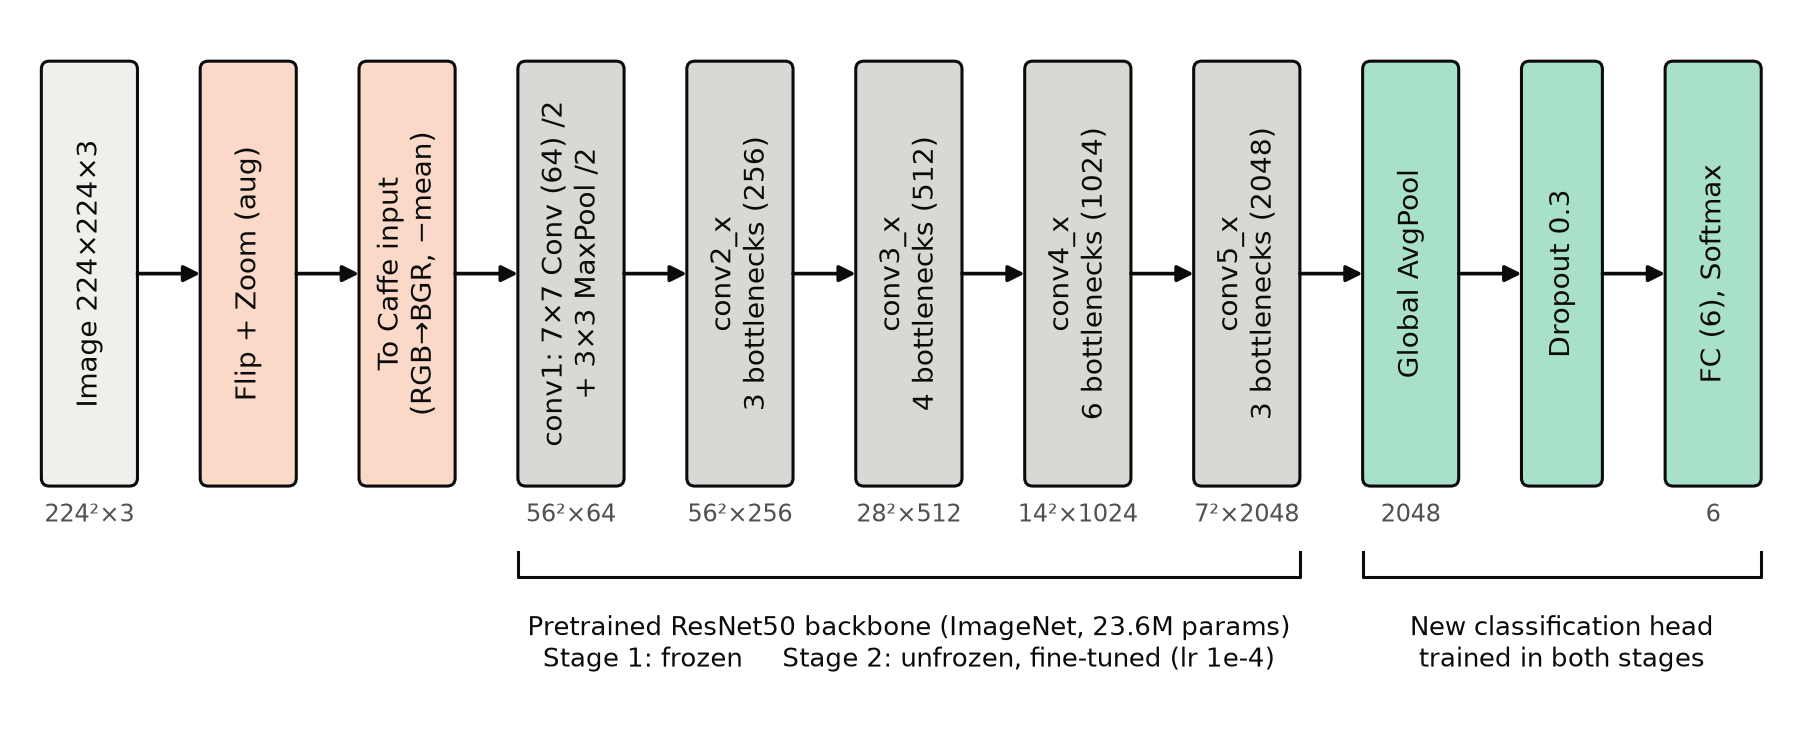
\includegraphics[width=0.95\textwidth]{resnet50_transfer.png}
\caption{Architecture of Model 3 (grey: pretrained backbone; green: new classification head).}
\label{fig:resnet}
\end{figure}

\textbf{Structure.} The third model reuses \textbf{ResNet50} \cite{he2016} pretrained on ImageNet \cite{deng2009},
loaded from \texttt{keras.applications} without its 1000-class top (Figure~\ref{fig:resnet}). The backbone is a
$7\times7$ stride-2 convolution and a max pooling followed by four stages of bottleneck residual blocks (3, 4, 6 and 3
blocks with 256, 512, 1024 and 2048 output channels), which turn a $224\times224\times3$ image into a
$7\times7\times2048$ tensor. On top of it we add a new head: global average pooling (2048 features), dropout 0.3 and a
6-unit softmax layer ($2048\cdot6+6=12{,}294$ parameters). In front of the backbone come the augmentation block and a
``to Caffe'' layer that undoes our ImageNet standardization, rescales to 0--255, swaps RGB to BGR and subtracts the
ImageNet mean (103.939, 116.779, 123.68), which is exactly the preprocessing used when the weights were pretrained.

The model is trained in two stages (Table~\ref{tab:resnet}):
\begin{itemize}
  \item \textbf{Stage 1 -- feature extraction.} The whole backbone is frozen (its BN layers also run in inference mode)
        and only the new head is trained, for at most 3 epochs with learning rate $10^{-3}$. This gives the head a
        sensible initialization, so that in stage 2 large random gradients do not damage the pretrained features.
  \item \textbf{Stage 2 -- fine-tuning.} All layers are unfrozen, the model is recompiled so that the optimizer sees the
        new trainable weights, and the whole network is trained for at most 10 more epochs with a ten times smaller
        learning rate, $10^{-4}$, weight decay $10^{-4}$ and early-stopping patience 3. The final model is the
        stage-2 checkpoint with the best validation macro-F1.
\end{itemize}

\begin{table}[htbp]
\centering\small
\caption{Parameters of Model 3 in the two training stages (*the 53{,}120 running statistics of the BN layers are never
trained by gradient descent).}
\label{tab:resnet}
\begin{tabular}{lrll}
\toprule
Part & Parameters & Stage 1 & Stage 2 \\
\midrule
ResNet50 backbone (ImageNet)      & 23{,}587{,}712 & frozen    & trainable* \\
New head (GAP, dropout, Dense 6)  & 12{,}294       & trainable & trainable \\
\midrule
\textbf{Total}                    & \textbf{23{,}600{,}006} & 12{,}294 trainable & 23{,}546{,}886 trainable \\
\bottomrule
\end{tabular}
\end{table}

\textbf{Why this design.} ResNet50 is the standard backbone for transfer learning: its ImageNet features (edges,
colours, textures, illumination) are useful for road scenes; it belongs to the same residual family as Model~2, which
makes the comparison ``own design vs.\ pretrained design'' fair; and with 23.6~M parameters it can be fine-tuned with
batch 32 on a 12~GB GPU. The head is kept minimal (GAP and one linear layer) so that the result reflects the pretrained
features rather than a large new classifier. The two-stage schedule protects the pretrained weights from the large
gradients of a randomly initialized head, and the smaller learning rate in stage~2 adapts the features instead of
overwriting them \cite{yosinski2014}. With 49{,}382 training images -- many for a transfer-learning task -- fine-tuning
the whole network rather than only the head is justified.

\FloatBarrier
% ------------------------------------------------------------------------------------------------ IV
\subsection{IV. Experimental Results}

\subsubsection{1. Results on the test set}
Table~\ref{tab:main} gives the results of the four trained models on the 8{,}841 test images (precision, recall and
F1-score are macro-averaged; the best value of each column is in bold).

\begin{table}[htbp]
\centering\small
\caption{Results on the test set.}
\label{tab:main}
\begin{tabular}{lccccc}
\toprule
Model & Accuracy & Precision & Recall & F1-score & Parameters \\
\midrule
Simple CNN                & 0.7559 & 0.5918 & 0.5953 & 0.5928 & 6.67 M \\
Simple CNN + Aug          & 0.7768 & 0.6213 & 0.6517 & 0.6333 & 6.67 M \\
Complex CNN + Aug         & 0.8098 & 0.6769 & \best{0.7177} & \best{0.6927} & 5.02 M \\
ResNet50 + Aug + Transfer & \best{0.8112} & \best{0.6924} & 0.6805 & 0.6817 & 23.60 M \\
\bottomrule
\end{tabular}
\end{table}

The two strongest models are close: the \textbf{complex CNN} has the best macro-F1 (0.6927) and macro recall,
\textbf{ResNet50} the best accuracy (0.8112) and macro precision; they differ by only 0.15 percentage points in
accuracy and 1.1 points in macro-F1. All models are far above the trivial baseline that always predicts the largest
class, night\_clear, which would reach 37.1\% accuracy and a macro-F1 below 0.10. For every model the accuracy is
12--16 points higher than the macro-F1. This gap is the signature of class imbalance: the three large classes are
recognized well and dominate the accuracy, while the small night\_unclear and dawn/dusk classes pull the macro average
down (Section IV.3). Table~\ref{tab:train} summarizes the training runs: for every model the best validation macro-F1
is within one point of the test macro-F1, so checkpoint selection did not over-fit the validation set.

\begin{table}[htbp]
\centering\small
\caption{Training summary (from the training logs; time on one RTX 3060, including validation after each epoch).}
\label{tab:train}
\begin{tabular}{lccccc}
\toprule
Model & Epochs run & Best epoch & Best val.\ macro-F1 & Test macro-F1 & Time (min) \\
\midrule
Simple CNN                & 18    & 13            & 0.5972 & 0.5928 & 17 \\
Simple CNN + Aug          & 19    & 14            & 0.6282 & 0.6333 & 31 \\
Complex CNN + Aug         & 21    & 16            & 0.6960 & 0.6927 & 94 \\
ResNet50 + Aug + Transfer & 3 + 8 & stage 2, ep.~5 & 0.6865 & 0.6817 & 81 \\
\bottomrule
\end{tabular}
\end{table}

\subsubsection{2. Learning curves}
\begin{figure}[htbp]
\centering
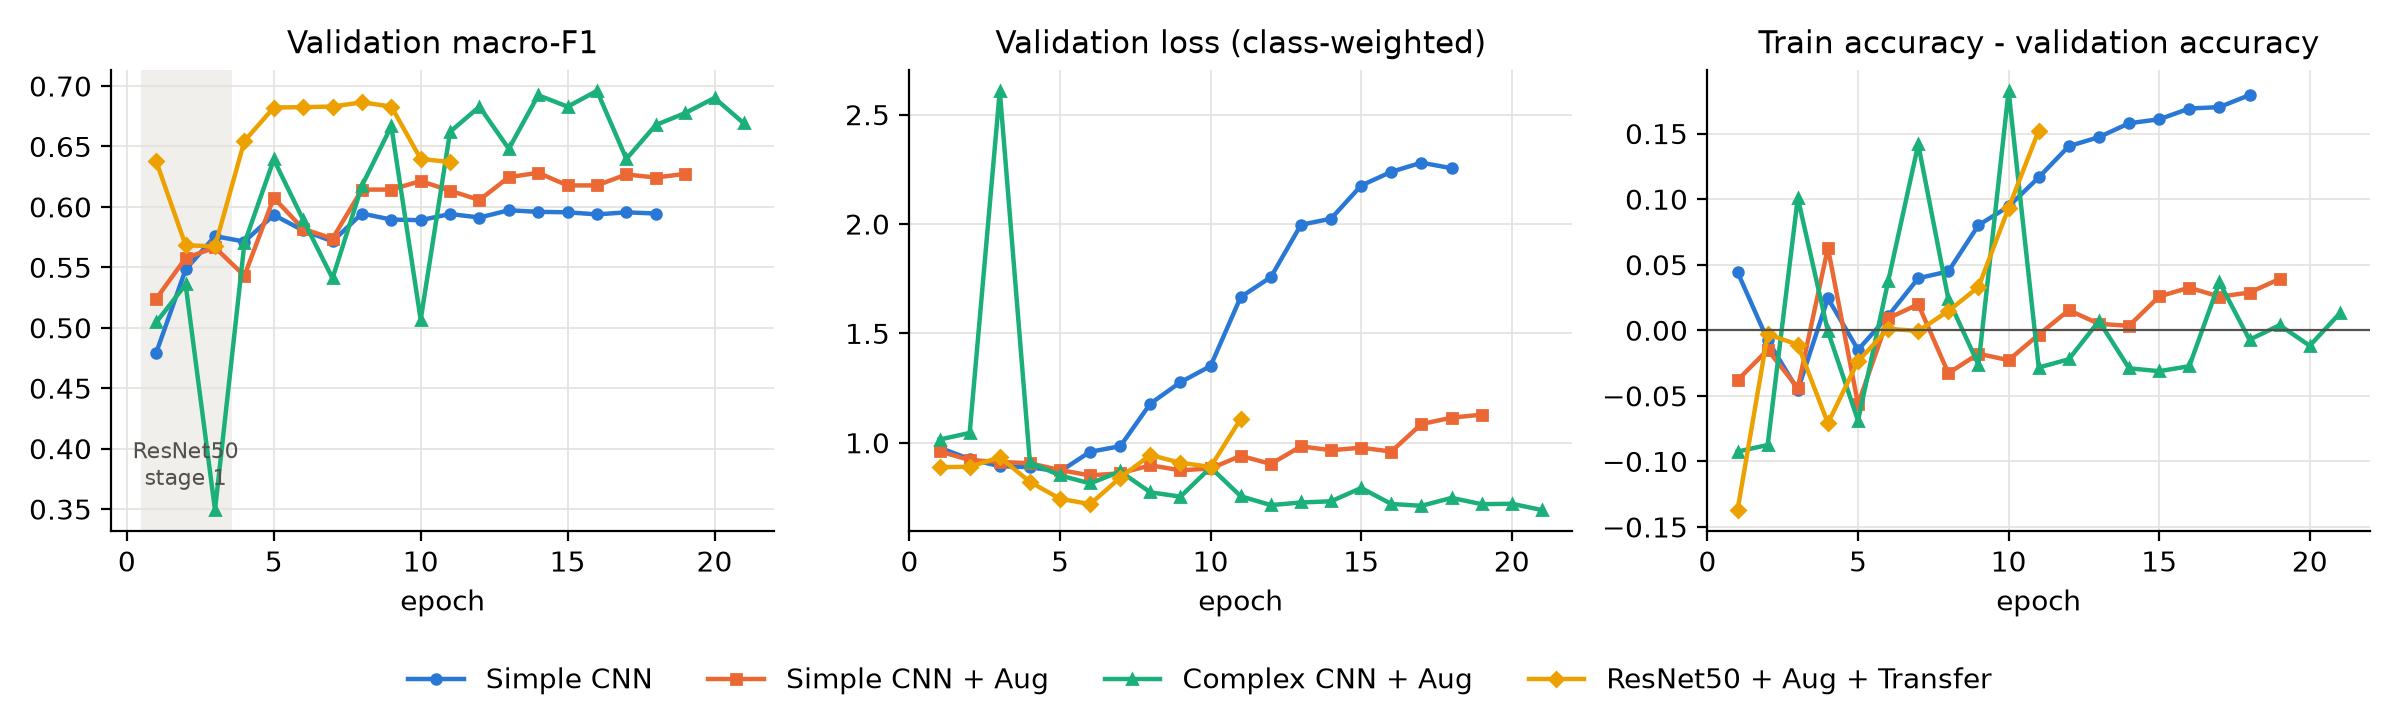
\includegraphics[width=\textwidth]{learning_curves.png}
\caption{Validation macro-F1, validation loss and over-fitting gap (training minus validation accuracy) per epoch,
from the training logs. For ResNet50, epochs 1--3 are stage 1 and epochs 4--11 stage 2.}
\label{fig:curves}
\end{figure}

Figure~\ref{fig:curves} shows how the four models were trained. The training accuracy is measured with augmentation
and dropout active, which is why it can be lower than the validation accuracy.
\begin{itemize}
  \item \textbf{Simple CNN without augmentation} over-fits strongly: the training accuracy climbs to 0.93 while the
        validation accuracy stays around 0.75, and the validation loss rises from 0.87 at epoch 5 to 2.26 at epoch 18.
        The 6.4-million-weight dense layer simply memorizes the training images.
  \item \textbf{With augmentation}, the same network reaches only 0.81 training accuracy after 19 epochs and its
        validation loss rises much less (from 0.85 to 1.13): augmentation acts as a strong regularizer.
  \item \textbf{Complex CNN:} training and validation accuracy stay close (0.79 and up to 0.81), so there is little
        over-fitting, thanks to batch normalization, global average pooling and weight decay. The validation metrics
        fluctuate strongly during the first 11 epochs (validation F1 0.35 at epoch 3 and 0.51 at epoch 10), a typical
        effect of batch normalization: the running statistics used at inference lag behind the quickly changing
        weights. The fluctuations fade after the learning rate is reduced at epochs 7 and 11.
  \item \textbf{ResNet50:} after a single epoch of stage 1 (frozen backbone, new head only) the validation accuracy is
        already 0.78, which shows that ImageNet features transfer well. Fine-tuning improves it to 0.82 within 2--5
        epochs, but then the training accuracy keeps rising to 0.90 while the validation loss increases: the
        23.5-million-parameter network starts to over-fit, early stopping ends training and the best checkpoint
        (stage-2 epoch 5) is restored.
\end{itemize}

\subsubsection{3. Per-class results}
Table~\ref{tab:perclass} gives the precision, recall and F1-score of every class and Figure~\ref{fig:cm} the confusion
matrices, normalized by row (each row shows how the test images of one true class are distributed over the predicted
classes).

\begin{table}[htbp]
\centering\footnotesize
\setlength{\tabcolsep}{3.5pt}
\caption{Precision / recall / F1-score per class on the test set (best F1 of each class in bold).}
\label{tab:perclass}
\begin{tabular}{lccccr}
\toprule
Class & Simple CNN & Simple CNN + Aug & Complex CNN + Aug & ResNet50 & Images \\
\midrule
daytime\_clear    & .802 / .813 / .807 & .836 / .802 / .819 & .864 / .814 / \best{.838} & .911 / .721 / .805 & 2{,}402 \\
daytime\_unclear  & .756 / .747 / .751 & .772 / .731 / .751 & .778 / .802 / \best{.790} & .697 / .878 / .777 & 1{,}862 \\
night\_clear      & .883 / .860 / .871 & .913 / .888 / .900 & .946 / .880 / .912 & .927 / .948 / \best{.937} & 3{,}279 \\
night\_unclear    & .374 / .437 / .403 & .496 / .557 / .525 & .564 / .736 / .639 & .677 / .649 / \best{.663} & 584 \\
dawndusk\_clear   & .432 / .455 / .443 & .426 / .597 / .497 & .498 / .677 / \best{.574} & .580 / .478 / .524 & 402 \\
dawndusk\_unclear & .305 / .260 / .280 & .285 / .337 / .308 & .411 / .397 / \best{.404} & .363 / .410 / .385 & 312 \\
\midrule
macro average     & .592 / .595 / .593 & .622 / .652 / .633 & .677 / .718 / \best{.693} & .692 / .681 / .682 & 8{,}841 \\
\bottomrule
\end{tabular}
\end{table}

\begin{figure}[htbp]
\centering
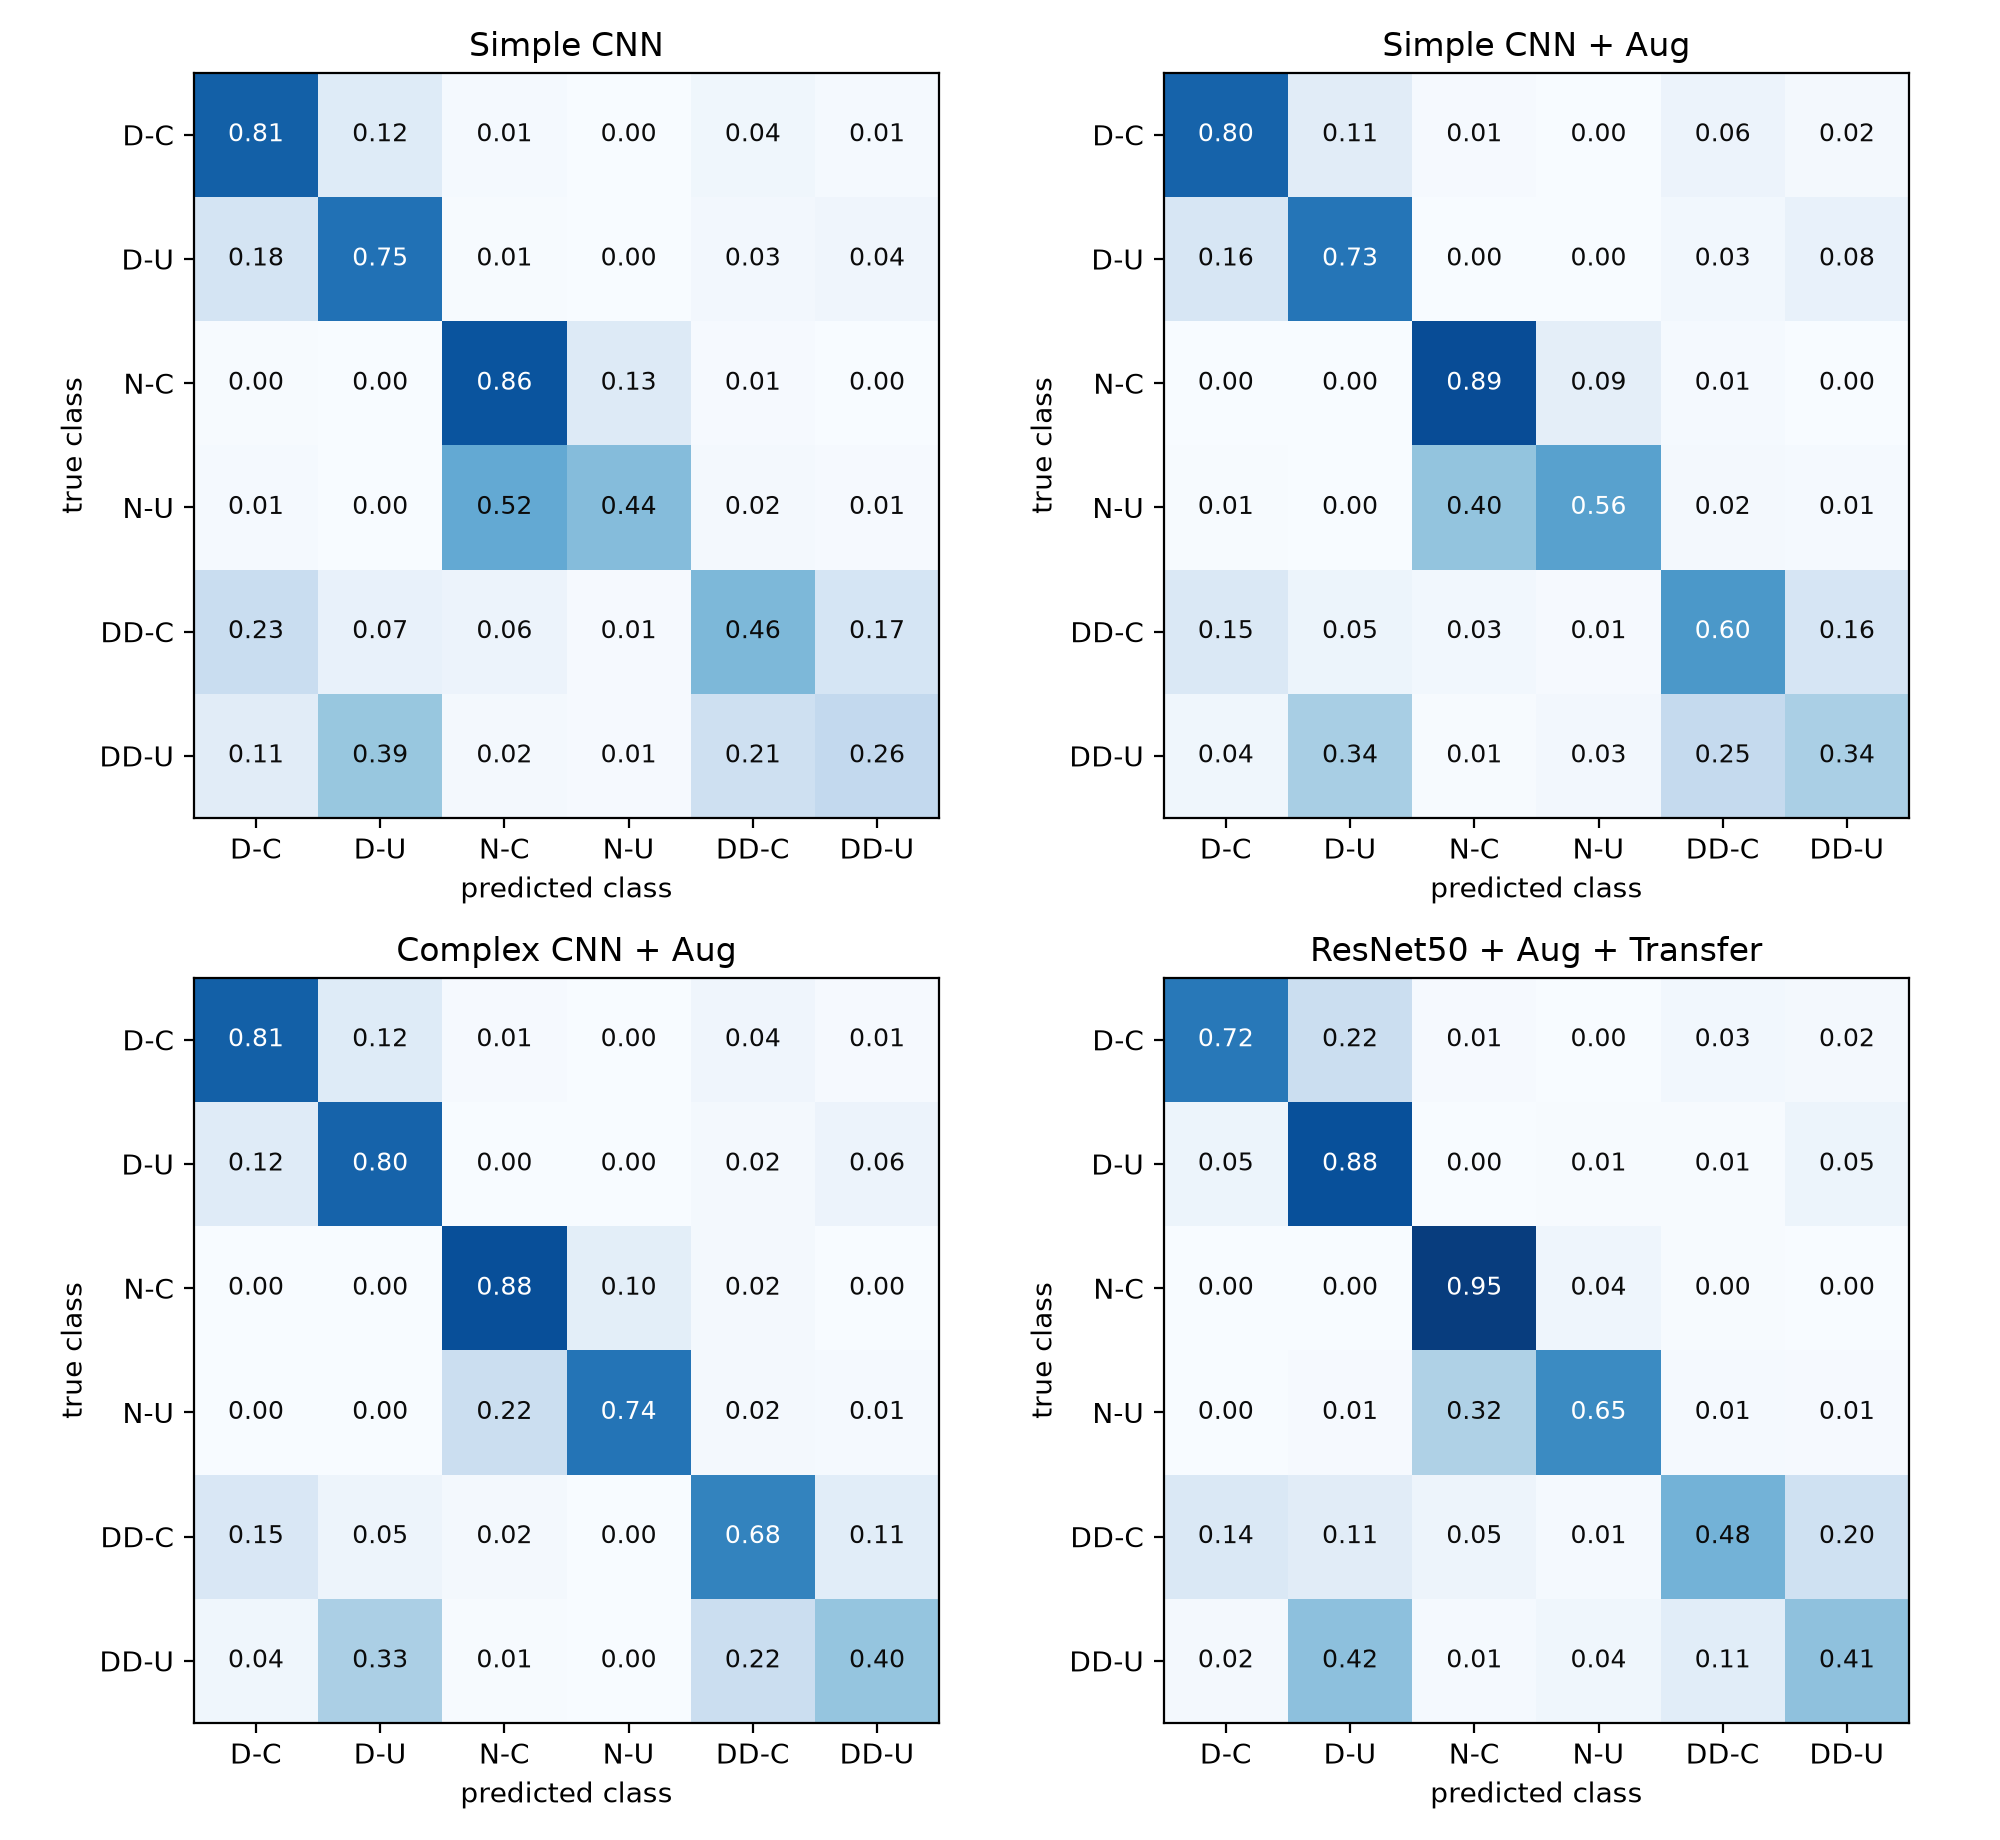
\includegraphics[width=0.62\textwidth]{confusion_matrices.png}
\caption{Row-normalized confusion matrices on the test set (D = daytime, N = night, DD = dawn/dusk; C = clear,
U = unclear).}
\label{fig:cm}
\end{figure}

\begin{itemize}
  \item The ranking of the classes is the same for all models. night\_clear is the easiest class (F1 0.87--0.94),
        followed by the two daytime classes (0.75--0.84). night\_unclear, dawndusk\_clear and dawndusk\_unclear are
        much harder; dawndusk\_unclear, the smallest class, stays below 0.41 for every model. The order follows both
        the class size and how ambiguous the class is visually.
  \item Every improvement helps the small classes most. From the simple CNN without augmentation to the complex CNN,
        the F1 of night\_unclear rises from 0.403 to 0.639 and that of dawndusk\_unclear from 0.280 to 0.404, while
        night\_clear only improves from 0.871 to 0.912. The class weights make the models bold on rare classes:
        their recall is often higher than their precision (complex CNN, night\_unclear: recall 0.74, precision 0.56).
  \item ResNet50 is the best model on both night classes (0.937 and 0.663), but it labels 22\% of the daytime\_clear
        test images as daytime\_unclear -- the largest single error of any model -- so its daytime\_clear recall is
        only 0.72. The complex CNN is more balanced and is clearly better on the two dawn/dusk classes (0.574 vs 0.524
        and 0.404 vs 0.385), which explains its higher macro-F1.
\end{itemize}

Because every class combines a time of day and a weather condition, the six-class predictions can be split into the
two underlying sub-tasks (Table~\ref{tab:subtasks}). \textbf{Time of day} is the easier sub-task: all models are right
about 92--93\% of the time, and night is recognized almost perfectly (97.5--98.9\%). Nearly all time-of-day errors
involve dawn/dusk: only 71\% of the dawn/dusk test images are assigned to a dawn/dusk class by the complex CNN (56\% by
the simple CNN without augmentation), and most of the others are predicted as daytime. \textbf{Weather} is harder
(81--86\%) and benefits most from augmentation (+3.0 points) and from the better architectures (+2.3 points).
Consequently, the most frequent six-class errors are weather errors within the same time of day: night\_clear
$\leftrightarrow$ night\_unclear and daytime\_clear $\leftrightarrow$ daytime\_unclear.

\begin{table}[htbp]
\centering\small
\caption{Accuracy on the two sub-tasks, derived from the six-class predictions.}
\label{tab:subtasks}
\begin{tabular}{lccc}
\toprule
Model & 6-class accuracy & Time of day (3 classes) & Weather (clear / unclear) \\
\midrule
Simple CNN                & 75.6\% & 92.3\% & 81.1\% \\
Simple CNN + Aug          & 77.7\% & 91.8\% & 84.1\% \\
Complex CNN + Aug         & 81.0\% & 93.3\% & 86.4\% \\
ResNet50 + Aug + Transfer & 81.1\% & 93.3\% & 86.4\% \\
\bottomrule
\end{tabular}
\end{table}

\subsubsection{4. Error analysis}
To see which weather conditions cause the errors, Table~\ref{tab:tags} breaks the weather part of the predictions down
by the original BDD100K weather tag.

\begin{table}[htbp]
\centering\small
\caption{Share of test images whose weather (clear / unclear) is predicted correctly, by original weather tag.}
\label{tab:tags}
\begin{tabular}{llrccc}
\toprule
Original tag & Merged label & Test images & Simple CNN + Aug & Complex CNN & ResNet50 \\
\midrule
clear         & clear   & 5{,}345 & 90.0\% & 90.0\% & 89.5\% \\
partly cloudy & clear   & 738     & 74.9\% & 75.5\% & 60.4\% \\
overcast      & unclear & 1{,}239 & 81.8\% & 84.3\% & 90.3\% \\
rainy         & unclear & 737     & 81.8\% & 87.0\% & 84.1\% \\
snowy         & unclear & 769     & 57.6\% & 75.4\% & 86.1\% \\
foggy         & unclear & 13      & 61.5\% & 46.2\% & 38.5\% \\
\bottomrule
\end{tabular}
\end{table}

\begin{itemize}
  \item \textbf{Clear} skies are easy (about 90\% for all models). \textbf{Partly cloudy} images, which we merged into
        \emph{clear}, are the hardest common tag: the complex CNN gets 75.5\% of them right and ResNet50 only 60.4\%.
        A sky full of clouds is visually close to an overcast sky, and this is exactly where ResNet50's
        daytime\_clear $\rightarrow$ daytime\_unclear errors come from; ResNet50 is in turn the best on overcast and
        snowy images.
  \item \textbf{Snowy} images improve the most with model capacity (from 58\% for the simple CNN to 75\% and 86\%):
        snow is often visible only as small patches at the roadside, a local cue that deeper networks capture better.
        \textbf{Foggy} images are too rare (143 in the whole dataset, 13 in the test set) to be learned.
  \item \textbf{Night:} since the sky cannot be seen in the dark, \emph{unclear} at night means rain or snow, and
        \emph{clear} means ``no visible precipitation''. Wet roads after rain and reflections of street lights look
        very similar to rain, which causes most night\_clear $\leftrightarrow$ night\_unclear errors.
  \item \textbf{Dawn/dusk} covers a continuum from a low sun in a bright sky to an almost dark street, and the boundary
        with daytime and night is subjective; depending on the model, 27--39\% of the dawn/dusk test images are
        predicted as daytime.
\end{itemize}

Figure~\ref{fig:errors} shows random misclassified test images of the complex CNN. Several of them are arguably label
noise or genuinely ambiguous: a scene labelled dawn/dusk that looks like an ordinary cloudy day, night scenes with wet,
reflective roads labelled clear, and images degraded by reflections of the dashboard on the windshield.

\begin{figure}[htbp]
\centering
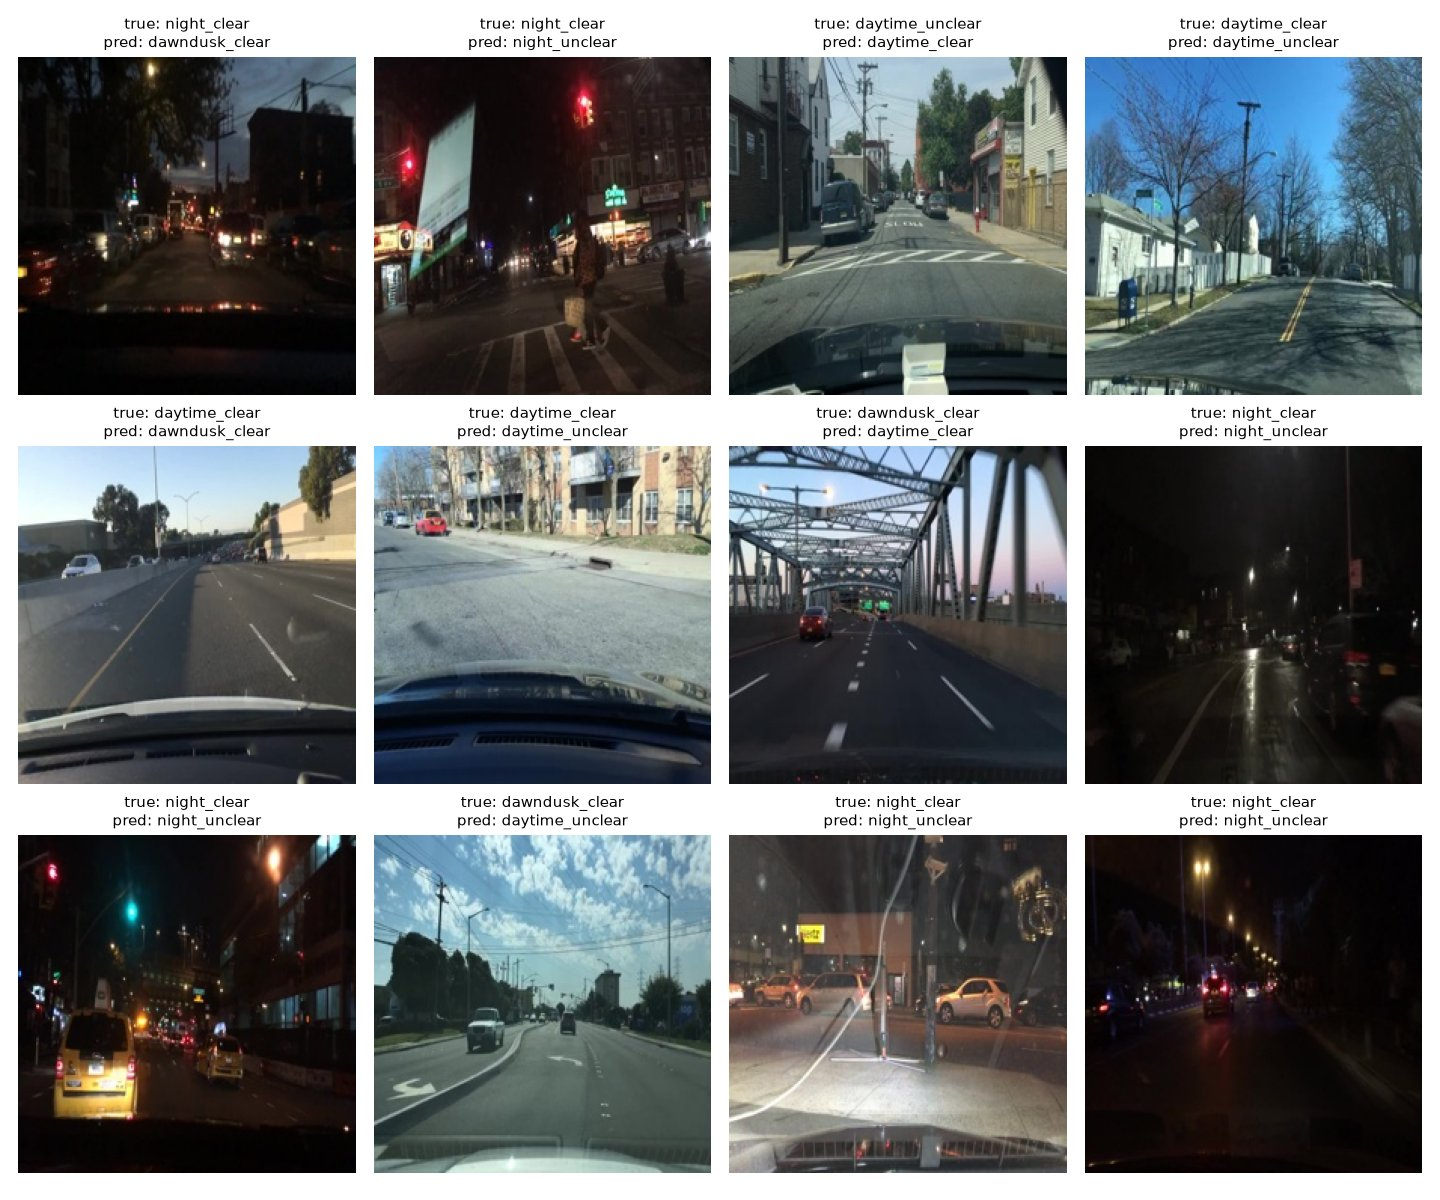
\includegraphics[width=0.56\textwidth]{errors.jpg}
\caption{Random misclassified test images of the complex CNN (true and predicted class above each image, shown at the
$224\times224$ input resolution).}
\label{fig:errors}
\end{figure}

\FloatBarrier
\subsubsection{5. Discussion}
\textbf{Effect of data augmentation (Simple CNN vs Simple CNN + Aug).} Adding only a horizontal flip and a small zoom
improves the accuracy by 2.1 points, the macro recall by 5.6 points and the macro-F1 by 4.1 points, with the same
architecture and number of parameters. The learning curves show why: augmentation greatly reduces over-fitting of the
large dense layer. Because the transformations were chosen to keep the label unchanged, they add variety without
adding label noise.

\textbf{Effect of CNN blocks (Simple CNN + Aug vs Complex CNN + Aug).} The complex CNN improves the accuracy by 3.3
points and the macro-F1 by 5.9 points while using 25\% fewer parameters. Batch normalization and residual shortcuts make
a deeper network trainable, and global average pooling replaces the huge dense layer, so capacity is spent on feature
extraction instead of on memorization. Table~\ref{tab:iter} also shows that the training configuration matters as much
as the architecture: the same blocks with a stride-1 stem and a higher learning rate either stopped early with a
macro-F1 of 0.638 or needed more than three times as long.

\textbf{Effect of transfer learning (Complex CNN vs ResNet50).} ResNet50 learns fastest -- even a linear head on frozen
ImageNet features reaches 0.78 validation accuracy after one epoch -- and it gives the highest accuracy and precision
and the best results at night. It does not, however, beat the complex CNN on macro-F1 (0.6817 vs 0.6927). Three reasons
are plausible: (i) ImageNet features are object-centric, whereas our classes depend on global photometric cues such as
illumination, sky colour and haze; (ii) with 23.6 million parameters the network over-fits after a few fine-tuning
epochs, and the short schedule and learning rates were not tuned; (iii) the squashed $224\times224$ input removes detail
such as raindrops on the windshield. Since each model was trained only once, a difference of about one point in
macro-F1 is within the variation that different random seeds can produce: the two models should be regarded as
comparable, with complementary strengths (ResNet50: night classes and precision; complex CNN: dawn/dusk classes and
recall).

\textbf{Cost.} On the RTX 3060 the simple CNN trains in 17--31 minutes, the complex CNN in 94 minutes and ResNet50 in 81
minutes. ResNet50 has 4.7 times more parameters than the complex CNN, so the complex CNN is also the cheaper model to
store and run. Overall, when all six classes matter equally (macro-F1, the main metric of this project), the complex
CNN is the best choice; when overall accuracy and precision matter more, ResNet50 is slightly better.

% ------------------------------------------------------------------------------------------------ V
\subsection{V. Conclusion}
This project addressed the classification of dashcam images from BDD100K into six classes that combine the time of day
(daytime, night, dawn/dusk) and the weather (clear, unclear). We built the dataset from the image-level tags (70{,}569
images after cleaning), designed a label-preserving preprocessing and augmentation pipeline with class-weighted training
for the strongly imbalanced classes, and trained and compared three CNNs and one ablation. The main results are:
\begin{itemize}
  \item The \textbf{complex CNN} built from residual ConvBlocks with BN, a stride-2 stem and global average pooling
        achieved the best macro-F1, \textbf{0.6927}, with an accuracy of 0.8098 and only 5.0 million parameters.
        \textbf{ResNet50} with two-stage fine-tuning achieved the best accuracy, \textbf{0.8112}, with a macro-F1 of
        0.6817. The simple CNN reached 0.7768 accuracy and 0.6333 macro-F1.
  \item Label-preserving data augmentation improved the simple CNN by 4.1 macro-F1 points and strongly reduced
        over-fitting; CNN blocks with batch normalization, shortcuts and global average pooling added another 5.9 points
        with fewer parameters; transfer learning gave the fastest convergence and the highest accuracy but not a better
        macro-F1.
  \item Time of day is recognized correctly about 93\% of the time and night almost perfectly; the remaining difficulty
        lies in dawn/dusk images and in the weather sub-task (about 86\%), especially for partly cloudy skies and for
        rain at night. The rare classes -- night\_unclear and the two dawn/dusk classes -- remain the hardest, partly
        because their labels are ambiguous.
\end{itemize}
\textbf{Limitations.} The time-of-day and weather tags of BDD100K are subjective and sometimes noisy. Images were
squeezed from 16:9 to a square $224\times224$ input, each model was trained once with a single seed, and no systematic
hyper-parameter search was carried out, so differences of about one point between models should be interpreted with
care. \textbf{Future work.} Possible improvements include two separate output heads for time of day and weather
(multi-task learning), higher-resolution or aspect-preserving inputs, more recent backbones such as EfficientNet or
ConvNeXt, losses designed for imbalanced data such as the focal loss, synthetic images for the rare dawn/dusk and foggy
conditions, an ensemble of the complex CNN and ResNet50, whose strengths are complementary, and using several frames of
the driving videos instead of a single image.

% ------------------------------------------------------------------------------------------------ references
\begin{thebibliography}{99}
\small
\setlength{\itemsep}{1pt}
\bibitem{goodfellow2016} I. Goodfellow, Y. Bengio, and A. Courville, \emph{Deep Learning}. Cambridge, MA, USA: MIT
  Press, 2016.
\bibitem{lecun1998} Y. LeCun, L. Bottou, Y. Bengio, and P. Haffner, ``Gradient-based learning applied to document
  recognition,'' \emph{Proc. IEEE}, vol. 86, no. 11, pp. 2278--2324, 1998.
\bibitem{krizhevsky2012} A. Krizhevsky, I. Sutskever, and G. E. Hinton, ``ImageNet classification with deep
  convolutional neural networks,'' in \emph{Advances in Neural Information Processing Systems}, vol. 25, 2012,
  pp. 1097--1105.
\bibitem{zhang2023} A. Zhang, Z. C. Lipton, M. Li, and A. J. Smola, \emph{Dive into Deep Learning}. Cambridge, U.K.:
  Cambridge University Press, 2023. [Online]. Available: \url{https://d2l.ai}
\bibitem{lin2014} M. Lin, Q. Chen, and S. Yan, ``Network in network,'' in \emph{Proc. ICLR}, 2014.
\bibitem{nair2010} V. Nair and G. E. Hinton, ``Rectified linear units improve restricted Boltzmann machines,'' in
  \emph{Proc. ICML}, 2010, pp. 807--814.
\bibitem{he2009} H. He and E. A. Garcia, ``Learning from imbalanced data,'' \emph{IEEE Trans. Knowledge and Data
  Engineering}, vol. 21, no. 9, pp. 1263--1284, 2009.
\bibitem{rumelhart1986} D. E. Rumelhart, G. E. Hinton, and R. J. Williams, ``Learning representations by
  back-propagating errors,'' \emph{Nature}, vol. 323, pp. 533--536, 1986.
\bibitem{kingma2015} D. P. Kingma and J. Ba, ``Adam: A method for stochastic optimization,'' in \emph{Proc. ICLR},
  2015.
\bibitem{loshchilov2019} I. Loshchilov and F. Hutter, ``Decoupled weight decay regularization,'' in \emph{Proc.
  ICLR}, 2019.
\bibitem{micikevicius2018} P. Micikevicius, S. Narang, J. Alben, G. Diamos, E. Elsen, D. Garcia, B. Ginsburg,
  M. Houston, O. Kuchaiev, G. Venkatesh, and H. Wu, ``Mixed precision training,'' in \emph{Proc. ICLR}, 2018.
\bibitem{srivastava2014} N. Srivastava, G. Hinton, A. Krizhevsky, I. Sutskever, and R. Salakhutdinov, ``Dropout: A
  simple way to prevent neural networks from overfitting,'' \emph{JMLR}, vol. 15, pp. 1929--1958, 2014.
\bibitem{ioffe2015} S. Ioffe and C. Szegedy, ``Batch normalization: Accelerating deep network training by reducing
  internal covariate shift,'' in \emph{Proc. ICML}, 2015, pp. 448--456.
\bibitem{shorten2019} C. Shorten and T. M. Khoshgoftaar, ``A survey on image data augmentation for deep learning,''
  \emph{J. Big Data}, vol. 6, no. 60, 2019.
\bibitem{simonyan2015} K. Simonyan and A. Zisserman, ``Very deep convolutional networks for large-scale image
  recognition,'' in \emph{Proc. ICLR}, 2015.
\bibitem{szegedy2015} C. Szegedy, W. Liu, Y. Jia, P. Sermanet, S. Reed, D. Anguelov, D. Erhan, V. Vanhoucke, and
  A. Rabinovich, ``Going deeper with convolutions,'' in \emph{Proc. IEEE CVPR}, 2015, pp. 1--9.
\bibitem{he2016} K. He, X. Zhang, S. Ren, and J. Sun, ``Deep residual learning for image recognition,'' in
  \emph{Proc. IEEE CVPR}, 2016, pp. 770--778.
\bibitem{huang2017} G. Huang, Z. Liu, L. van der Maaten, and K. Q. Weinberger, ``Densely connected convolutional
  networks,'' in \emph{Proc. IEEE CVPR}, 2017, pp. 4700--4708.
\bibitem{deng2009} J. Deng, W. Dong, R. Socher, L.-J. Li, K. Li, and L. Fei-Fei, ``ImageNet: A large-scale
  hierarchical image database,'' in \emph{Proc. IEEE CVPR}, 2009, pp. 248--255.
\bibitem{yosinski2014} J. Yosinski, J. Clune, Y. Bengio, and H. Lipson, ``How transferable are features in deep
  neural networks?'' in \emph{Advances in Neural Information Processing Systems}, vol. 27, 2014, pp. 3320--3328.
\bibitem{yu2020} F. Yu, H. Chen, X. Wang, W. Xian, Y. Chen, F. Liu, V. Madhavan, and T. Darrell, ``BDD100K: A
  diverse driving dataset for heterogeneous multitask learning,'' in \emph{Proc. IEEE/CVF CVPR}, 2020,
  pp. 2636--2645.
\bibitem{lu2014} C. Lu, D. Lin, J. Jia, and C.-K. Tang, ``Two-class weather classification,'' in \emph{Proc. IEEE
  CVPR}, 2014, pp. 3718--3725.
\bibitem{chollet2015} F. Chollet \emph{et al.}, ``Keras,'' 2015. [Online]. Available: \url{https://keras.io}
\bibitem{paszke2019} A. Paszke \emph{et al.}, ``PyTorch: An imperative style, high-performance deep learning
  library,'' in \emph{Advances in Neural Information Processing Systems}, vol. 32, 2019, pp. 8024--8035.
\bibitem{pedregosa2011} F. Pedregosa \emph{et al.}, ``Scikit-learn: Machine learning in Python,'' \emph{JMLR},
  vol. 12, pp. 2825--2830, 2011.
\bibitem{repo} N. T. Q. Dat, B. H. G. Huy, T. D. Anh, and N. D. Tuan, ``BDD100K weather classification -- source
  code,'' GitHub, 2026. [Online]. Available:
  \url{https://github.com/imissu-datntq/BDD100K-weather-classification}
\bibitem{kaggle} solesensei, ``BDD100K dataset (Kaggle mirror).'' [Online]. Available:
  \url{https://www.kaggle.com/datasets/solesensei/solesensei_bdd100k}
\bibitem{bddsite} Berkeley DeepDrive, ``BDD100K: A large-scale diverse driving video database.'' [Online]. Available:
  \url{https://bdd-data.berkeley.edu}
\end{thebibliography}

\end{document}
